\chapter{A Data Acquisition System for the Test Beam}
\label{chap:II-3-test-beam}

  During the ongoing process of the development of the DAQ system, the electronics has been tested in two test beams organised in Fall 2014 and Fall 2015. The first test beam, ran with the first prototype of the DAQ, aimed at proving the feasability of the architecture of the system, not focusing on data taking from the provided pion and muon beam but rather on usability. As the results were encouraging, the second version of the electronics was developped involving a complete redesign of the hardware, firmware, and software. Therefore, we will mainly focus on the second test beam, which electronics is described in the previous chapter, during which abundant data was recorded showing both excellent results for the detectors and the DAQ system. \\

  In this chapter, we present the firmware and software developments done for the DAQ system for the test beams followed by the analysis of the recorded data. First, we will present the firmware architecture of the OH and the GLIB to better understand the global layout of the system and the features that have been implemented to control the components. Then we will move on to the back-end applications developped to control and monitor the DAQ system and read out data. Finally, after a presentation of the layout of the test beam setup and its characteristics, we will show the results obtained after analysis of the recorded data.

  \section{Architecture of the OptoHybrid Firmware}

    The most important function of the OptoHybrid is to transfer data between the VFAT2s and the GLIB. Downwards, from the off-detector to the on-detector electronics, it transfers slow control requests and fast commands while upwards it sends the trigger and tracking data back to the back-end system. Next to the handling of the basic VFAT2 functionnalities, it must also handle the optical links and a couple of programmable registers which control the system. Furthermore, procedures that were previously implemented in software and required extensive computanionnal time have been moved to firmware in order to speed up the system. \\

    Although rather complex, the firmware of the OptoHybrid can be decomposed in six blocks: the fast commands, the trigger data, the tracking data, the slow control, the calibration routines, and the optical links. Eventough these blocks separatly will be presented, they are tighlty interconnected using a wishbone-like architecture for intercommunication.

    \subsection{Internal Communication Through a Wishbone-Like Architecture}

      Wishbone is an open-source communication protocol used in many projects to enable data transfer between ICs. A light version of the protocol has been implemented in the OptoHybrid to link the various modules of the system. The latter are divided in two categories: masters which initiate requests, and slaves which provide responses. The link between the two is done through a switching hub which redirects the requests to the appropriate slaves by using a 32-bit-long address space mapped to the various modules. By design, multiple masters can interact simultaneously with different slaves allowing for parrallelism in the system. \\

      A request form a master is composed of four signals: a flag signaling the presence of a request, a write-enable bit to indicate the nature of the request (read or write), a 32-bit-long address to which the request will be redirected, and an optionnal 32-bit-long data field in case the request is a write operation. The response from a slave consists of: an ackownledgment signal, a 4-bit-long error status in case the operation failed, and an optionnal 32-bit-long data field holding the response to read requests. A programmable timeout has also been implemented to avoir blocking operation. Some components implement both a master and a slave module in order to be able to receive requests and propagate them to various other modules. \\

      Communication done through the wishbone-like protocol is used mainly for slow control or non-time-critical operations as the latency of a transaction is not fixed. Indeed, the switching hub implements a waiting list functionnality which allows two masters to address the same slave at the same time by storing one of the requests in memory and awaiting for the slave to finish the other transaction.

    \subsection{Encoding Fast Commands}

      Fast commands such as L1As, Resyncs, BC0s, etc can originate from various sources. In normal data taking runs, the AMC13 receives the TTC signals, forwards them to the microTCA AMC which in turn transmits them to the OptoHybrid. When data taking is stopped and calibration runs are performed, the routines implemented in the OptoHybrid are ran and require fast commands. To this end, the TTC signals can also be generated locally using the T1 generator block. This entity can generate L1As, Resyncs, BC0s, and CalPulses in three different ways: send a single command a given number of times at fixed interval, send a CalPulse followed by a L1A with a fixed delay, or send a programmable pattern involving all the commands. Finally, the two remaining sources of TTC commands, and more precisly L1As, are either a loopback from a given VFAT2 trigger bits directly to all the VFAT2s (self-triggering) or the signals coming from an external component through a debugging header on the OptoHybrid. \\

      The switching between the various sources is done by setting a register through slow control operations. Once the source has been selected, the commands are forwarded to the VFAT2s and encoded on the T1 signals. Each command is composed of three bits clocked at 40 MHz. An additionnal feature has been added to the L1A line to throttle the trigger signals when working in high rate environments. Through registers, the operator can select to send only a fraction of the received commands to not overload the VFAT2 buffers and allow for correct readout of the chip.

    \subsection{Formatting Trigger Data}

      Each of the 24 VFAT2s transmits eight trigger bits per BX. These are regroupped using a logic OR in the DAQ system of the test beam  thus yielding 24 bits. The trigger information is used for calibration routines and forwarded over debugging headers to an external electronics crate. As the number of external connections is limited, only six trigger bits can be send thus requiring the need for a selection mechanism controller by programmable registers.

    \subsection{Acquiring Tracking Data}

      Upon reception of a L1A, the VFAT2 transfers the selected event from its SRAM1 to SRAM2 and then to an encoder which serialises the data. Each event is 192 bits long followed by two idle bits and clocked at 40 MHz. This means that it takes 194 BXs to read out one event and that the VFAT2 cannot handle trigger rates higher than $\approx$ 200 kHz without experiencing an overflow of the buffers. The data is pushed out of the VFAT2 automatically and formatted according to the pattern shown in Table \ref{tab:II-3-vfat2-tk-format}. The top left bits are Most Significant Bits (MSBs) which are pushed out first and the bottom right bits or the Least Significant Bits (LSBs) which come in last. The first four bits of the first three 16-bit-long words are constant values. These are completed by the BC which increments at each clock cycle, the EC which counts the number of received L1As, four flags which hold information on the status of the buffers, and a chip ID unique to each VFAT2. Following are the 128 bits reflecting the hit information on each channel. Finally, the VFAT2 uses a Cyclic Redundancy Check (CRC) on 16 bits to detect errors. The CRC uses all other 176 bits to encode its data but does not provide a way to correct errors. \\

      \begin{table}
        \begin{tabularx}{\textwidth}{C{1}}
          \textbf{VFAT2 tracking data} \\
          {
          \begin{tabularx}{0.5\textwidth}{|C{1}|C{1}|C{1}|}
            \hline
            \multicolumn{3}{|c|}{15 \hfill 0} \\ \hline
            1010 & \multicolumn{2}{|c|}{BC[11:0]} \\ \hline
            1100 & EC[7:0] & Flags[3:0] \\ \hline
            1110 & \multicolumn{2}{|c|}{Chip ID[11:0]} \\ \hline
            \multicolumn{3}{|c|}{Channel data x8} \\ \hline
            \multicolumn{3}{|c|}{CRC} \\ \hline
          \end{tabularx} }
        \end{tabularx}
        \caption{??}
        \label{tab:II-3-vfat2-tk-format}
      \end{table}

      Next to the data line, each VFAT2 provides a DataValid line which is pulled high when the bits coming out of the VFAT2 are valid. However, due to the limited number of pins connecting the GEB and the OptoHybrid, this signal has been left unconnected for all but six VFAT2s. Therefore, data is constantly shifted in a 194 bits (192 bits of data and 2 idle bits) serial-to-parrallel converter and analyzed. When the fixed pattern of 12 bits is seen, a flag is raised signaling the presence of potential data. The data packet is split up in its various elements and the CRC is recomputed and compared against the received CRC. Two additionnal flags respectivly hold the results of the comparation of both CRCs indicating if the data is valid or not, and a logic OR of all 128 channel to indicate if the packet contains a hit or not. In theory, only packets with valid CRCs could be transmitted to the back-end electronics. However, sending all packets offer the possibility to identify recurring errors in the CRCs computation and offers the possibility to correct them offline. \\

      In parallel to the decoding of the data packets, the OptoHybrid maintains its own BC and stores the value of the counter in a buffer each time a L1A is received. When the decoding modules report they have detected data, a concentrator module aggragates the information from all available VFAT2s. Every packet received within a window of 10 BX is assigned to the same event to which the value of the corresponding BC is appended. The assembled event is stored in a large buffer to be latter sent over the optical links to the GLIB. \\

      To prevent positions either not equipped with VFAT2 Hybrids or that are noisy to generate fake data, a 24-bit-long register allows to mask individual positions to ignore any packets it generates. Next to this, each decoding module is equipped with two counter respectivly counting the number of valid and invalid packets.

    \subsection{Controlling and Monitoring the Systems}

      The OptoHybrid is used to control itself through wishbone and the VFAT2s through I2C. The slow control of the OptoHybrid mainly consists in selecting TTC command sources, setting the trigger throttling, reading out counters, etc. These operations are performed to control the data flow and the functionning of the DAQ system itself. Commands sent to the VFAT2s on the other hand have direct impact on the physics of the data taking through the biais of the analog front-end readout. \\

      To communicate with the VFAT2s, six I2C controllers are implemented in the firmware of the OptoHybrid, one per sector on the GEB. Each controller can access four VFAT2s which are identified using three resistors that can be installed on the GEB. VFAT2 uses a modified I2C protocol which uses the same frame format as the official one but a different addressing scheme. The official I2C data frame is shown in Figure \ref{fig:II-3-i2c}. The master starts by sending seven address bits which are used to identify the slave it wants to talk to, followed by a read/write bit. After the slave acknowledged the request, eight bits are sent from the master to the slave in case of a write operation followed by a slave acknowledgment, or the opposite in case of a read operation. For the VFAT2, the first three bits of the address are used to select the chip that is addressed by the master while the four remeaning bits are used to select the register that needs to be accessed. This addressing scheme allows the OptoHybrid to access up to 16 registers on the VFAT2s. However, each VFAT2 holds 16 primary registers and 136 extended registers. The extended registers are accesses using two primary pointer registers: one set to point to an extended register, and one to read/write the data in said register. Thus, in order to perform a transaction on a primary register, only one operation is necessary, while two are required to access extended registers. \\

      \begin{figure}[h!]
        \centering
        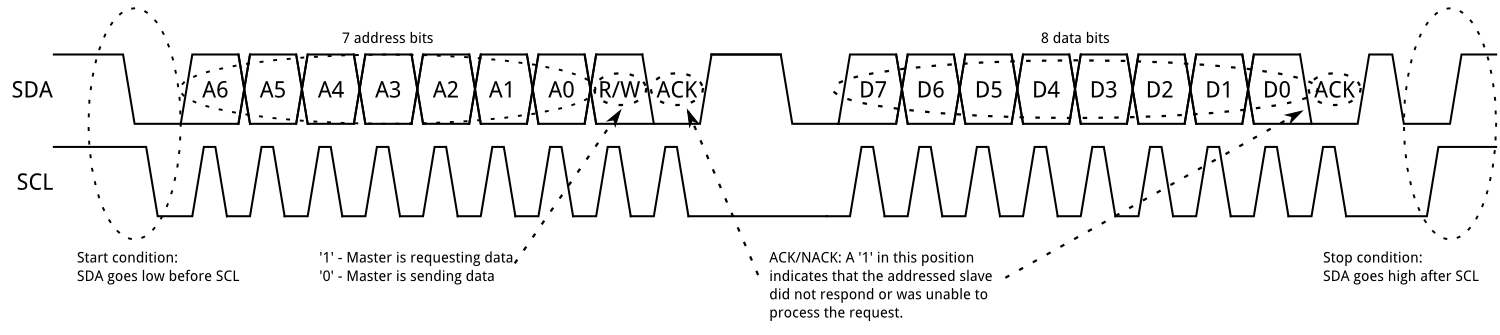
\includegraphics[width=\textwidth]{img/II-3-test-beam/i2c.png}
        \caption{??? \cite{I2C}.}
        \label{fig:II-3-i2c}
      \end{figure}

      To make this process transparent to the user and flatten out the address space of the VFAT2s, the OptoHybrid maps the primary registers from addresses 0 to 16 and the extended registers from addresses 17 to 152. When performing a transaction with the extended registers, the I2C controllers automatically run the double addressing scheme. \\

      Next to the basic I2C controllers, an extended I2C controller was developped to abstract individual addressing and allow request broadcasting. This module forwards I2C requests to all selected VFAT2s at once to configure the entire system in parallel. A programmable register allows to leave out given VFAT2s from the broadcast while a buffer stores the result of the operations.

    \subsection{Calibrating the Systems}

      The calibration routines have been ported from software to firmware in order to increase their speed of operation and reduce the number of requests that need to be performed. The routines are as follows: a threshold scan which measures the noise on the strips as a function of the threshold of the VFAT2s, a latency scan which allows to select the correct BX when receiving L1As, and a s-curve scan which characterize the response of the strips as a function of the collected charge and threshold. \\

      \paragraph{The threshold scan} is used to scan each VFAT2 for noise. For each threshold value set on the VFAT2, the percentage of events displaying a hit is recorded and taken as the percentage of noise. A graph can be obtained showing the noise decrease as the threshold increases yielding a point at which the system can be operated with minimal noise. The threshold scan can be operated using trigger information on the 128 strips as a whole or on individual strips using tracking data. For the latter, the T1 generator is used as trigger source to generate data as these runs being performed when the beam is off. No relation between a L1A and physical event is needed to study the noise on the system. \\

      \paragraph{The latency scan} allows to determine the best latency value to be set in a VFAT2. The latency is the time difference, in number of BX, between the time of arrival of a L1A and the time at which the related event was stored in the VFAT2 buffer. This module is operated when the particle beam is on and triggers are generated by an external source such as a Photomultiplier (PM) placed in front of the detector. For each value of the latency, the OptoHybrid counts the ratio of events with hits over the total number of events. For a noiseless VFAT2 with 100\% detection efficiency, the ratio would be 0\% outside the correct latency window and 100\% inside. The size of the window can be adjusted by changing the length of the monostables output in the VFAT2s. \\

      \paragraph{The s-curve scan} is part of the calibration routines performed for the qualification of the VFAT2s. It yields the response of the VFAT2 strips to an injected charge pulse according to the threshold. It is used in conjunction with the T1 generator which send a CalPulse followed by a L1A at fixed interval, thus with known latency. The use and results obtained for this module are further detailled in Chapter \ref{chap:II-5-qualification}.

    \subsection{Optical Communication with the Off-Detector Electronics}

      The link between the OptoHybrid and the off-detector electronics are the optical links from which two are used: one for the trigger data and fast commands, and one for the tracking data and slow control. Each optical fibre is connected to an SFP+ transceiver which contains the Light Emitting Diode (LED) that drives the link. The SFP+ module is in turn connected to a Gigabit Transceiver X (GTX) block inside the FPGA which is a dedicated component that can handle high-speed serial communications.

      \paragraph{The GTX module} is in charge of the serialization/deserialization of high-speed data. A schematic diagram of the functions it provides ir shown in Figure \ref{fig:II-3-gtx}. The GTX handles both the transmission and reception of data. From the FPGA logic, it receives a parallel vector of bits containing the raw data. The raw data enters the Transmit FIFO which acts as a buffer before the Line Encoding module. The latter uses an eight-bit/ten-bit (8b/10b) encoding scheming which is a standard in high-speed communications. 8b/10b encodes every eight bit word on ten bits according to a predefined table. It has the particularity that whatever combination of words might be sent, no more than five successive '0's or '1's will arise in the serial stream. This ensures line balancing: the fact that the electric lines between the GTX and the SFP+ module will remain at an average voltage and not drift to a logic '1' or '0' over time, thus requiring a longer fall or rise time of the signals. 8b/10b also offers a set of K-characters which are unique patterns of bit that can never arise randomly in the stream. Those characters are used to detect the beginning of a frame and allow the receiver to align correctly. Finally, after the encoding of the data frame is done, it is serialized and transmitted to the SFP+ module over differential pairs. \\

      \begin{figure}[h!]
        \centering
        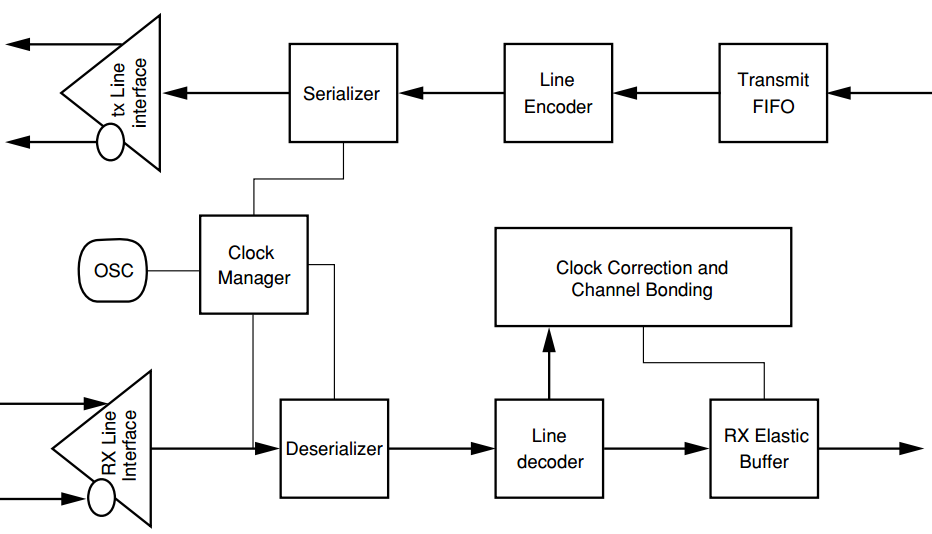
\includegraphics[width=\textwidth]{img/II-3-test-beam/gtx.png}
        \caption{??? \cite{GTX}.}
        \label{fig:II-3-gtx}
      \end{figure}

      The receiver essentially follows the opposite path as the transmitter except for the Clock Managment block. The 8b/10b encoding offers one more advantage which is the possibility to recover a clock from the data stream itself, technique called Clock Data Recovery (CDR). In high-speed signal design, small variations in the clock frequency between the transmitter and the receiver can lead to discrepancy in the read out data. To avoid this, the receiver can tune the frequency of the clock of its deserializer using the transitions of the bits in the incoming stream to align its phase to the data. The GTX block further provides the obtained recovered clock to the FPGA to use in the logic. Correct alignment of the data is checked using the K-characters in the stream.

      \paragraph{The fixed latency link} is used to transmit trigger data from the OptoHybrid to the GLIB and receive the fast commands. Of the 64 bits that the downlink transmits, 16 are used to align the serial bit stream on the receiving side and four others are used to encode the four fast commands that the VFAT2 understands. The other 44 bits are not used and left to constant zeros. The uplink uses a 16 bit header to align the stream to which it appends the 24 triggers bits coming from the logic-OR of the VFAT2s. These patterns repeat at 40 MHz as data changes every BX.

      \paragraph{The variable latency link} is used to transmit and receive slow control commands and to transmit the tracking data of one VFAT2 at the time to the GLIB. As only one VFAT2 was exposed to the beam at any given time during the test beam, reconstructing and sending the full event was not a necessity for the DAQ system. In both directions, a given frame format is constantly sent using two bits in the header to indicate the presence of a valid slow control request and valid VFAT2 tracking data in case of the uplink. The two data formats are shown in Table \ref{tab:II-3-data-format}. Both send a 16 bit header to align the link followed by the frame data. As can be seen in the table on the left, the OptoHybrid receives requests from the optical link which are then converted to wishbone-like requests by the logic. The optical link module is one of the wishbone masters that controls the system and which responses are forwarded back to the GLIB.

      \begin{table}
        \begin{tabularx}{\textwidth}{C{1}C{1}}
          \textbf{GLIB to OptoHybrid frame} & \textbf{OptoHybrid to GLIB frame} \\
          {
          \begin{tabularx}{0.4\textwidth}{|C{1}|}
            \hline
            15 \hfill 0 \\ \hline
            Header \\ \hline
            Request address (MSB) \\ \hline
            Request address (LSB) \\ \hline
            Request data (MSB) \\ \hline
            Request data (LSB) \\ \hline
            CRC \\ \hline
          \end{tabularx} }
          &
          { \begin{tabularx}{0.4\textwidth}{|C{1}|}
            \hline
            15 \hfill 0 \\ \hline
            Header \\ \hline
            VFAT2 data x14 \\ \hline
            Response data (MSB) \\ \hline
            Response data (LSB) \\ \hline
            CRC \\ \hline
          \end{tabularx} }
        \end{tabularx}
        \caption{??}
        \label{tab:II-3-data-format}
      \end{table}

      \subsection{System Summary}

        The aim of the OptoHybrid firmware is to provide a communication medium between the VFAT2s and the off-detector electronics and to speed up the calibration routines by implementing them closer to the detector. The developments that have been listed in this chapter are targeted at the OptoHybrid v2a and the configuration of the system ran during the test beams. Modifications have to be brought for the final system altough the foundations of the firmware have been solidly laight out.

  \section{Architecture of the GLIB Firmware}

    The GLIB development group at CERN provides a system firmware which controls the onboard components, handles the communication with the MCH, and implements the logic to decode IPBus requests. This code is similar to the operating system in which the users runs their applications by adding custom firmware. The latter is system specific and up to the user to develop. In our application, the firmware we developped for the GLIB is in charge of the buffering of the tracking data until it is read out by the application, and the forwarding of the IPBus requests over the optical link to the OptoHybrid. Other than that, the GLIB holds a couple of counters which monitor the status of the optical links and the number of requests performed. However, the firmware of the GLIB has been designed to be able to handle two OptoHybrids in parallel, seemlessly allowing the user to switch from one to another at any time.

    \subsection{The Tracking Data Readout}

      The GLIB acts as buffer for the tracking data it reads out from the OptoHybrids and decodes from the optical links. It stores the VFAT2 events until the control and monitoring application reads them out through IPBus. In case the buffers reach their full occupancy, new events are discarded and flags are raised. The buffers can hold up to 16,383 VFAT2 events per OptoHybrid connected and the system has been tested and proven to work without overflows up until L1A rates of 200 kHz, the maximum rate the VFAT2s can handle.

    \subsection{The IPBus Controller and Slaves}

      The IPBus decoding procedure is much similar to the wishbone system implemented on the OptoHybrid. According to the address contained in the request, the GLIB selects the slave it needs to address. Each request is made of a flag signaling the presence of a request, a read/write bit reporting the type of operation, a 32-bit-long address field, and an optionnal 32-bit-long data field populated with data in case of a write operation. The IPBus response is composed of an acknoledgment and error flag to signal the validity of a response, and an optionnal 32-bit-long data field containing the read data. By design, each IPBus request is decomposed in single read or write operations. Therefore, even if the software performs a read request of multiple addresses at once, IPBus slaves will still see this as multiple sequential read operations on single addresses. This in term propagates to the OptoHybrid wishbone requests which originate from IPBus requests meaning that no more than one wishbone request coming from the GLIB is present at any time in the system. As a majority of the requests have to be forwarded to the OptoHybrid, an entire address space of the GLIB is mapped to the former. These are handled by an IPBus slave connected to the GTX blocks of the GLIB. This module encodes the request according to the data format on the left in Table \ref{tab:II-3-data-format} and awaits for a response before signaling the IPBus controller.

  \section{The Control and Monitoring Application}

    The first version of the control and monitoring application that communicated with the system was based on a series of Python scripts running PyChips, a Python implementation of IPBus provided with the GLIB source code. Each script was developped to run a specific task and needed to be ran over and over again. This was feasable for the first test beam during which only the system was tested for small amounts of time, but not for the second one that was ment to collect data. Therefore, we developped a web application based on NodeJS \cite{NODEJS} as server technology, SocketIO \cite{SOCKETIO} for the client/server exchange, AngularJS \cite{ANGULARJS} as front-end framework, and Bootstrap \cite{BOOTSTRAP} as design framework.

    \subsection{Architecture of the Application}

      NodeJS is a JavaScript (JS) runtime that has the ability to run JS code outside the context of a web browser. It extendeds JavaScript from its original use in web content to a wide range of applications by enabling it to manipulate files, data streams, etc. The most common use for NodeJS is the implementation of a web server that has the property to be much more reactive than other infrastructures. Where classic server structures display a blocking behavior, meaning they only handle one request at the time blocking the queue of incoming demands, NodeJS is event driven and thus non-blocking. For example, if a client requests a file, NodeJS will transfer the request to the operating system and continue to respond to other client as long as the file is not served. Interactions are thus more reactive and allow to easily implement a real-time control and monitoring system. Along side the NodeJS server that serves the content of our web application, we also implemented a version of IPBus in JS. The latter allows the server to execute IPBus requests on the GLIB and readout the response. \\

      To link the client side controlled by the user and the server side which sends requests to the GLIB, the SocketIO project is used. It is an abstraction layer on the fairly new WebSocket technology which adds sockets to web browsers and allows for fast communication with servers by bypassing the HTTP protocol. When the client changes settings in its web browser, SocketIO transfers the request to NodeJS which in turn creates an IPBus packet. When the GLIB responded to the request, the server transfers the response back to the client which can handle the data as it likes. \\

      To handle data in a dynamic and convenient way, the web pages use Bootstrap and AngularJS. Bootstrap is a design framework which provides simple and readable themes to layout the pages. The content of the page on the other hand is managed by AngularJS which is a front-end JS framework. It helps rendering dynamic content in function of the data received from the server. Actions can be triggered or disabled according to the state of the system, data can be updated live, etc. It renders the user experience more fluid and enjoyable by providing a usable set of actions and an efficient navigation through the control pages.

    \subsection{Controling the Systems}

      The control over the GLIB, OptoHybrids, and VFAT2s is done through four pages which screenshots are shown in Figure \ref{fig:II-3-app-monitoring}. The top-left picture displays the home page of the application which provides an overview of the status of each system. The left panel displays the firmware version of the GLIB and OptoHybrids; the middle panel gives the occupancy of the GLIB readout buffers, which are here signaled as full through the use of a red flag, and the status of the various modules of the OptoHybrid; finally, the right panel lists the VFAT2s that are turned on in green, turned off in red, and missing in gray. By clicking on any of the elements, the user is redirected to the corresponding system control page. \\

      \begin{figure}[h!]
        \centering
        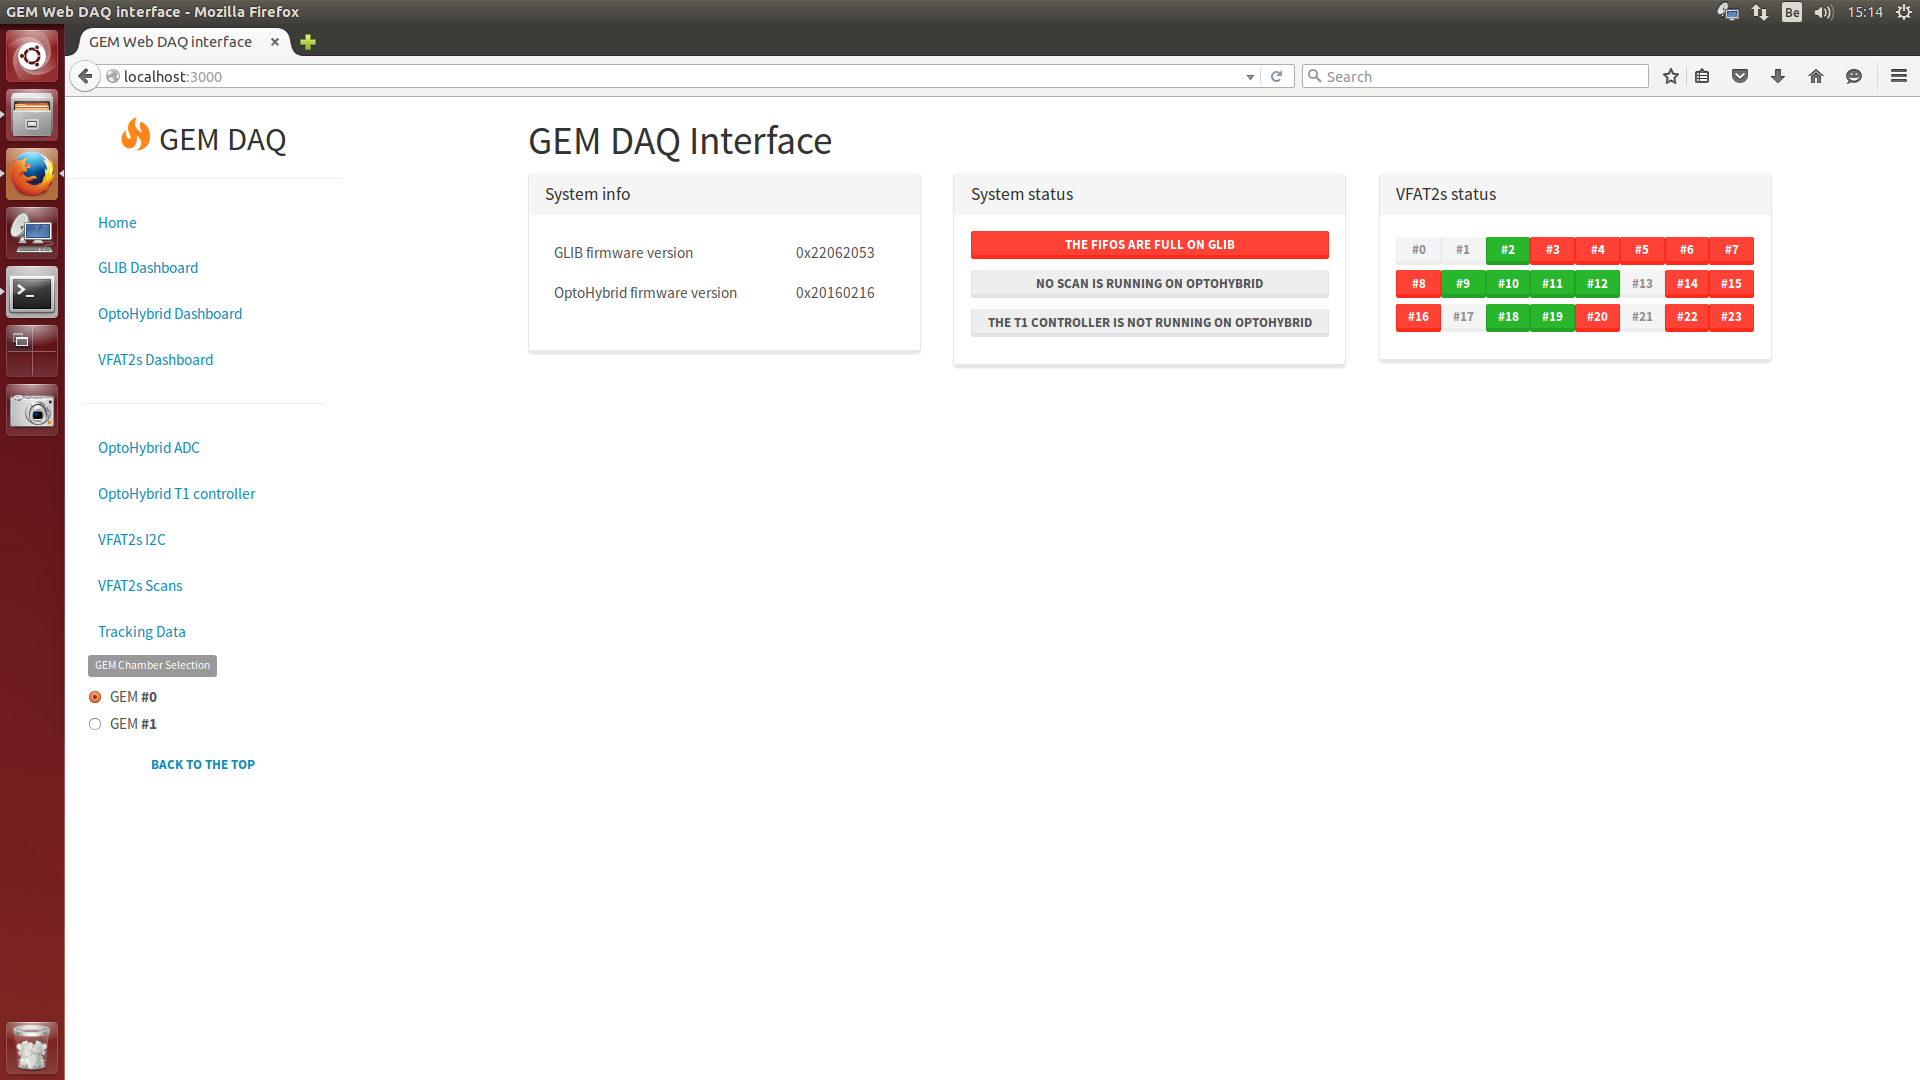
\includegraphics[width=0.49\textwidth]{img/II-3-test-beam/app-home.png}
        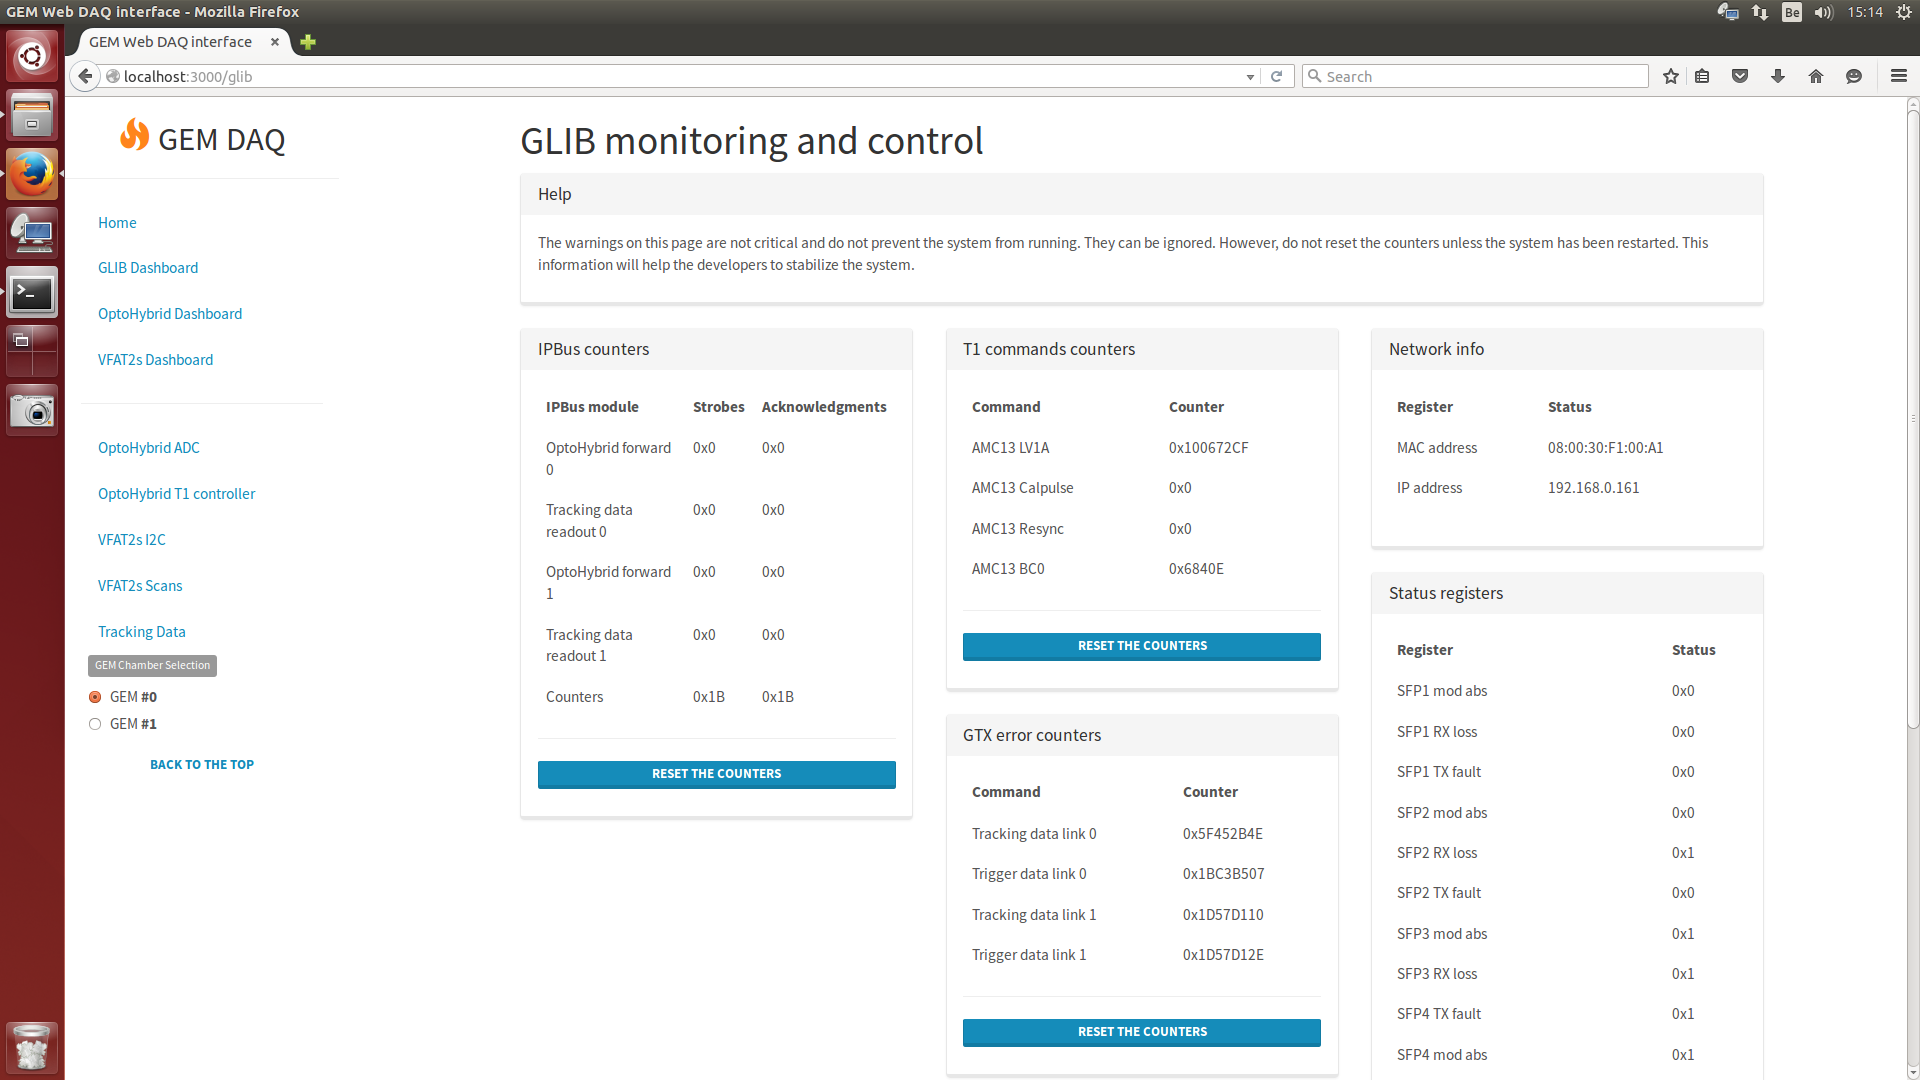
\includegraphics[width=0.49\textwidth]{img/II-3-test-beam/app-glib.png} \\
        \vspace*{0.3cm}
        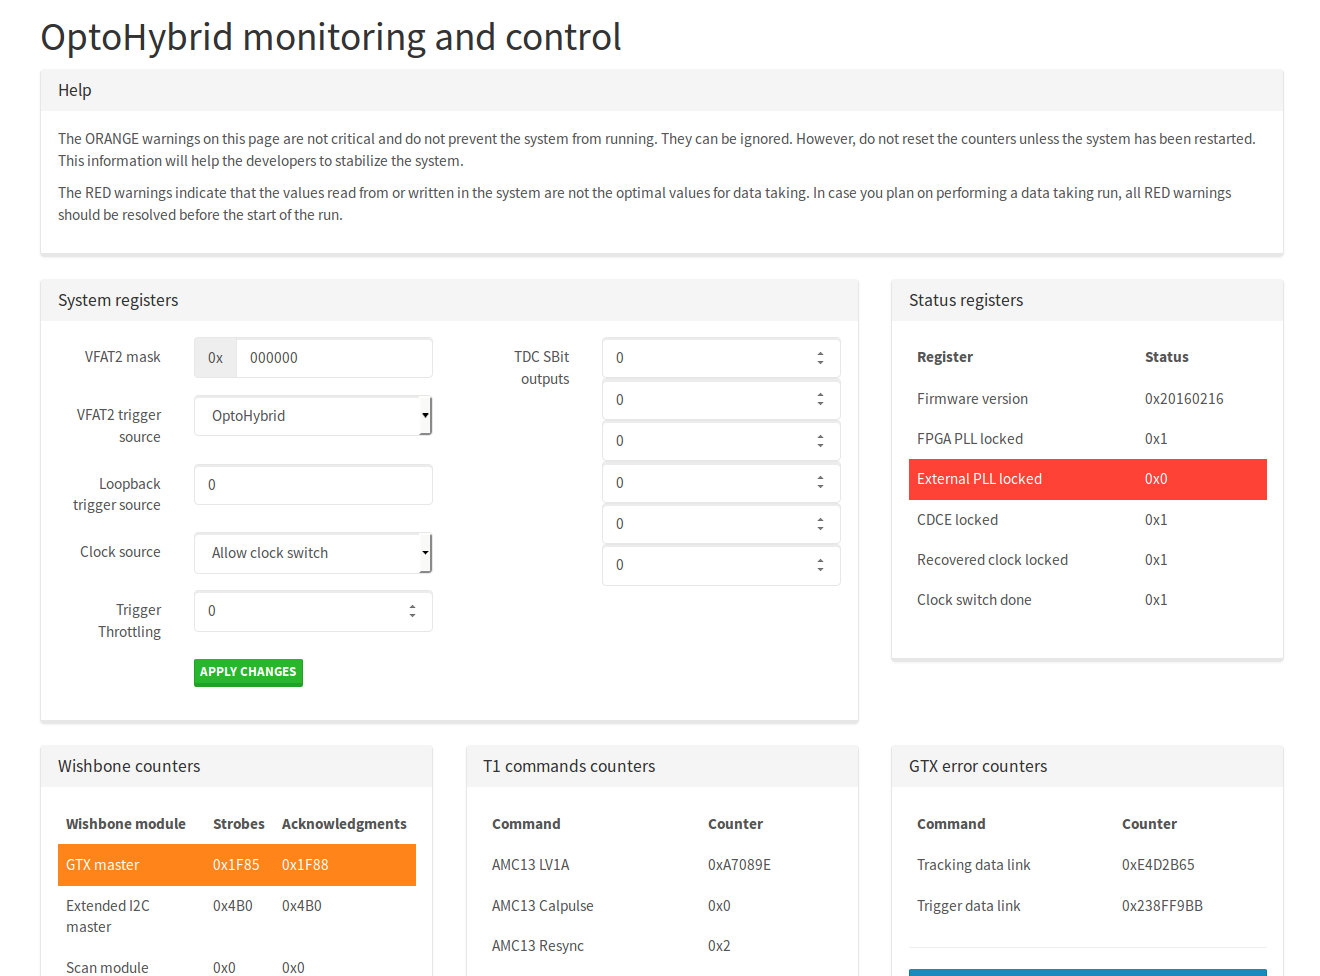
\includegraphics[width=0.49\textwidth]{img/II-3-test-beam/app-oh.png}
        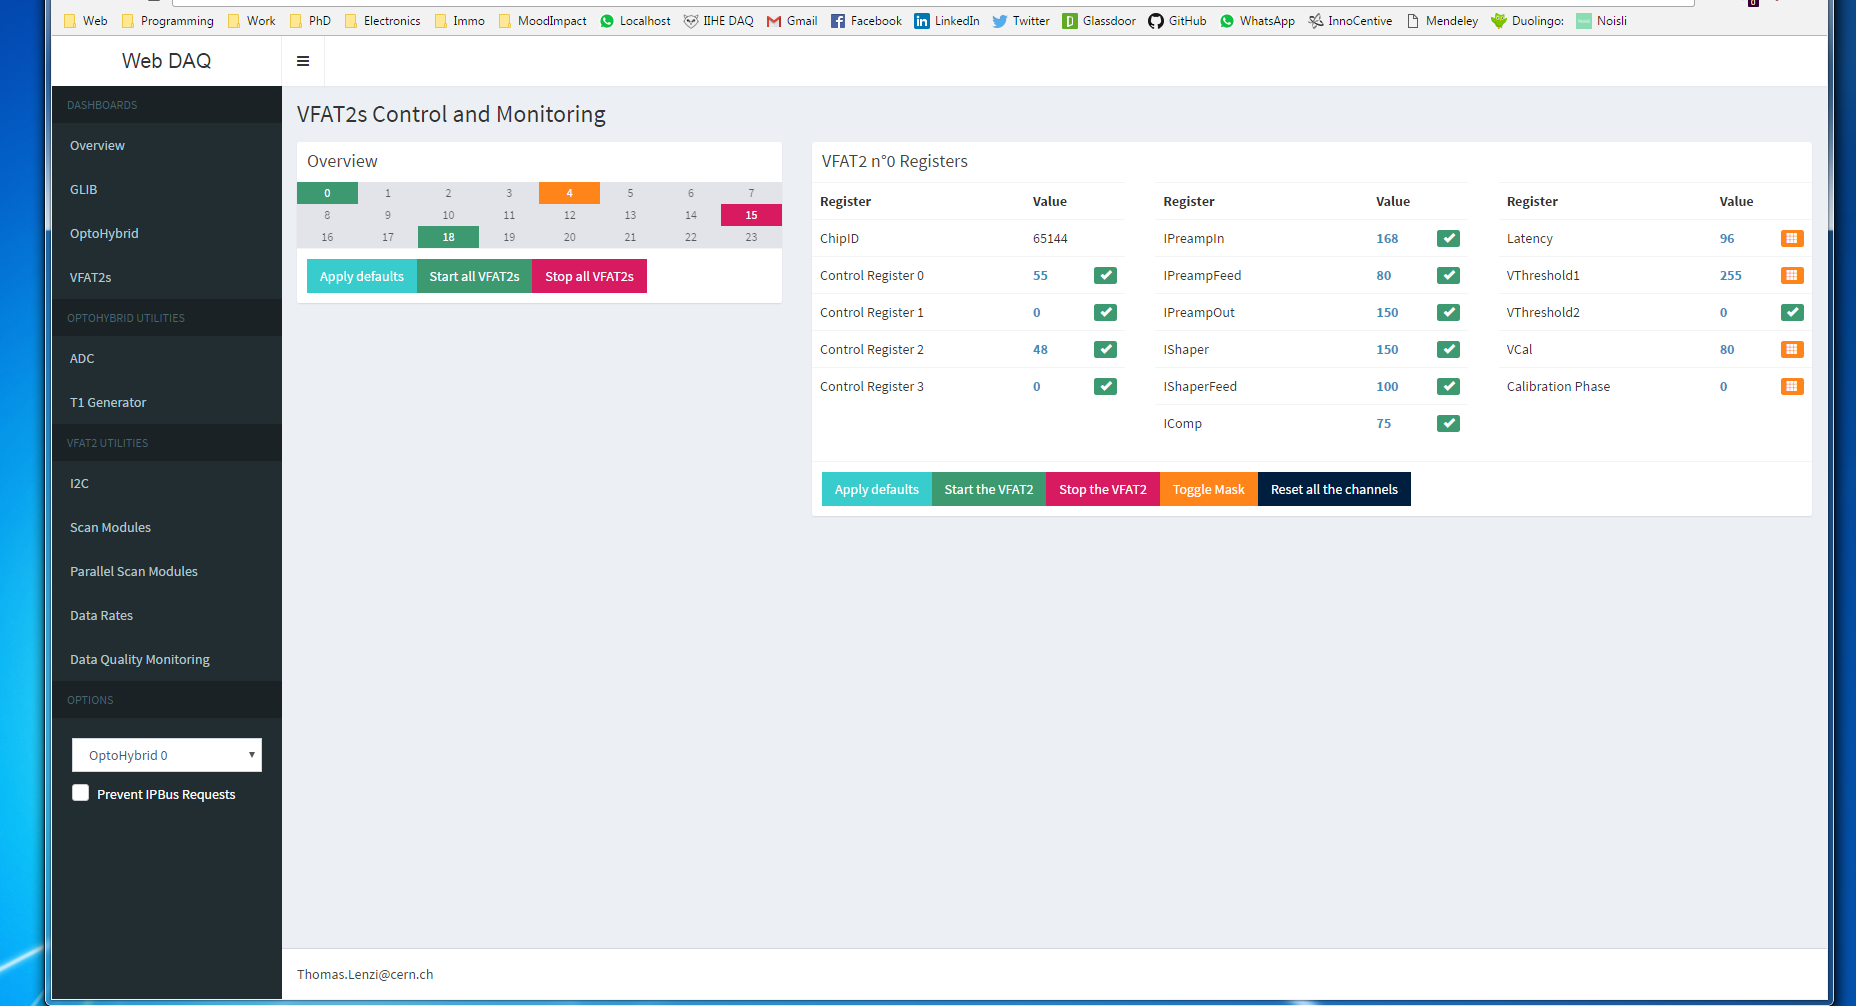
\includegraphics[width=0.49\textwidth]{img/II-3-test-beam/app-vfat2.png}
        \caption{???}
        \label{fig:II-3-app-monitoring}
      \end{figure}

      The control page of the GLIB is shown in the top-right corner. The information it contains is mainly related to counters which allow to see, for example, the number of requests sent to the OptoHybrid and the number of responds received. It also counts the number of errors detected on the optical link providing a quantitative value of the health of the link. \\

      The OptoHybrid page, shown in the bottom-left corner, provides more information and control options to the user. The top-left part of the page is used to modify system register controlling the trigger source, clock source, trigger information sent over the debugging header, etc. This is where the user can change the type of ongoing run by going from a data taking run using external triggers to a calibration run using internally generated triggers. The panel directly on the right provides status information on the various clocking ressources in the FPGA. By default, the OptoHybrid uses the onboard oscillator to power the system and the optical links. As communication is established with the GLIB, the GTXs provide the recovered clock from the link which is the system clock. When the latter is stable, the OptoHybrid can decide to switch from its onboard clock to the system clock in order to be synchronuous with the whole DAQ system. This operation can be prohibited, forced, or allowed by the user, which can also chose to use an external clock provided through the debugging header. These clocking options are usefull for the test beam setup where the clock can be provided externally to synchronize with other electonics equipment. Finally, the bottom part of the page display counter values for the wishbone request, fast commands, link errors, etc. Note that when a discrepancy is observed between two correlated counters, a warning flag is raised as can be seen in the bottom-left of the picture. \\

      Finally, the control page of the VFAT2s, shown in the bottom-right of the figure, gives access to the most significant registers of the front-end chips. It provides a sumarry of the on/off/absent status of each VFAT2 on the GEB and, by clicking on an individual slot, the value of each register as shown in the panel on the right. Default settings for the registers are saved in memory and compared to the current values, raising warnings when they differ and allowing the user to correct them. The user can also control all the VFAT2s at once by applying the default settings or turning them on or off at the same time. In the bottom panel, control buttons allow to mask individual VFAT2s in case they generate noise or send corrupted tracking data. Two counters monitor the number of valid (with a correct CRC) and invalid packets each position has sent.

    \subsection{Fast and Slow Control of the VFAT2s}

      The fast control or T1 generator is controlled by a dedicated page, displayed in the left of Figure \ref{fig:II-3-app-control}, which allows to select the type of commands to generate, the pattern to send, and the delay between two pulse. The slow control of the VFAT2s handled by the I2C modules and the extended I2C controller is managed by another page shown in the right. The slow control commands can either target a single VFAT2 as shown in the left panel or an entire set of chips as can be seen in the right panel. In case of a single command, the response is shown inline. For multiple operations, a table of results is shown indicating the value and the corresponding VFAT2. To help the user, the accessible registers are named rather than listed using their address.

      \begin{figure}[h!]
        \centering
        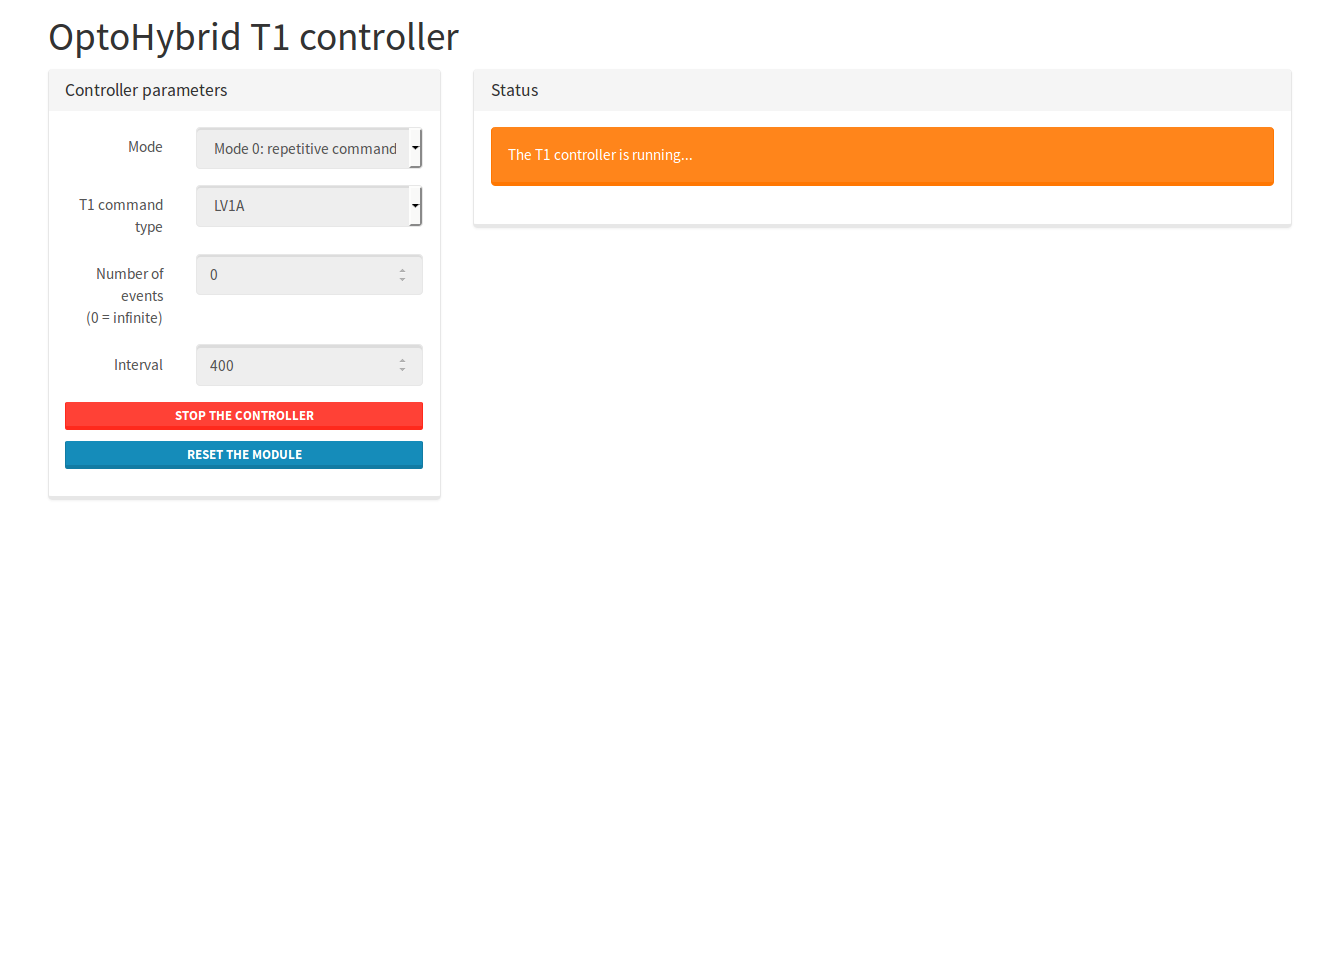
\includegraphics[width=0.49\textwidth]{img/II-3-test-beam/app-t1.png}
        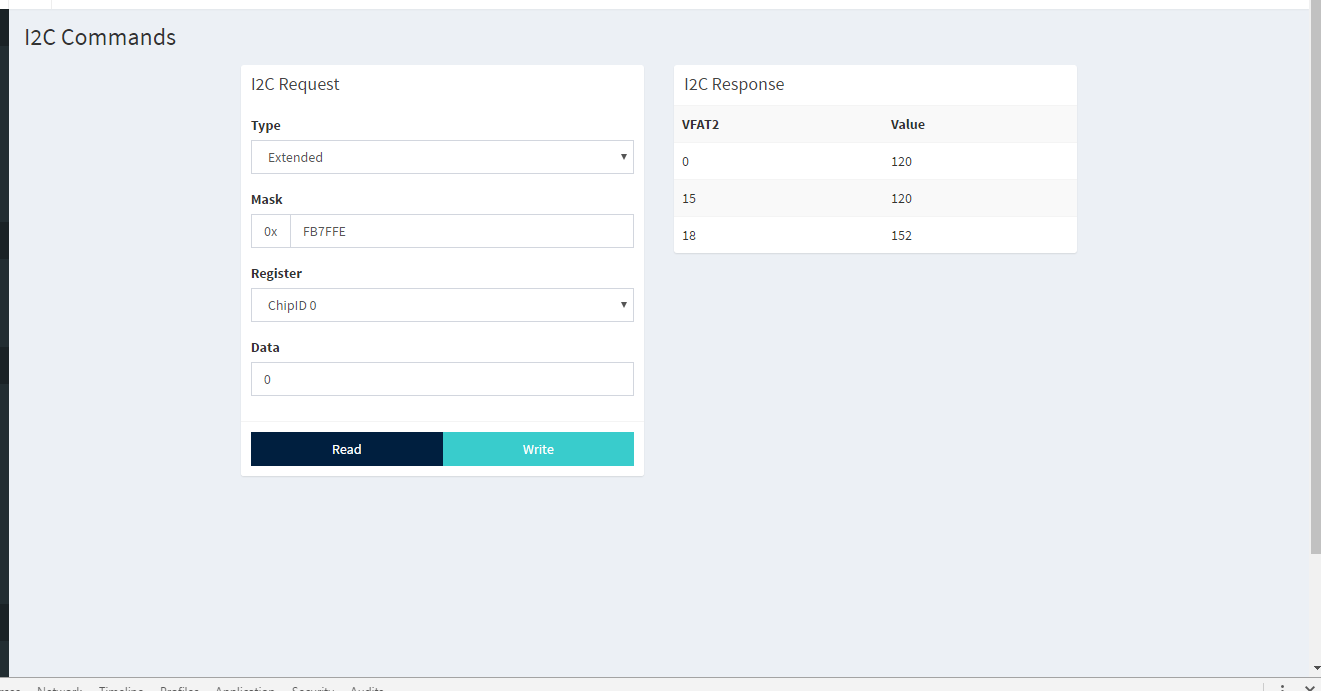
\includegraphics[width=0.49\textwidth]{img/II-3-test-beam/app-i2c.png}
        \caption{???}
        \label{fig:II-3-app-control}
      \end{figure}

    \subsection{Calibrating the VFAT2s}

      The calibration of the VFAT2s is done through a dedicated page which regroups the various operations that can be performed on the chip. Figure \ref{fig:II-3-app-calibration} is a screenshot of the application runing a threshold scan on one of the VFAT2s. The left panel allows the user to select all the required parameters such as the type of scan, the range of the scan, the number of events per point, etc. Once the parameters are entered, the user starts the scan and waits for it to finish in firmware. When done, a graph displays the results in the right panel. The user can than dynamically change VFAT2 settings by clicking on a point of the graph to, for example, select the most appropriate threshold or latency value. Furthermore, the user can save the data points to disk for offline analysis.

      \begin{figure}[h!]
        \centering
        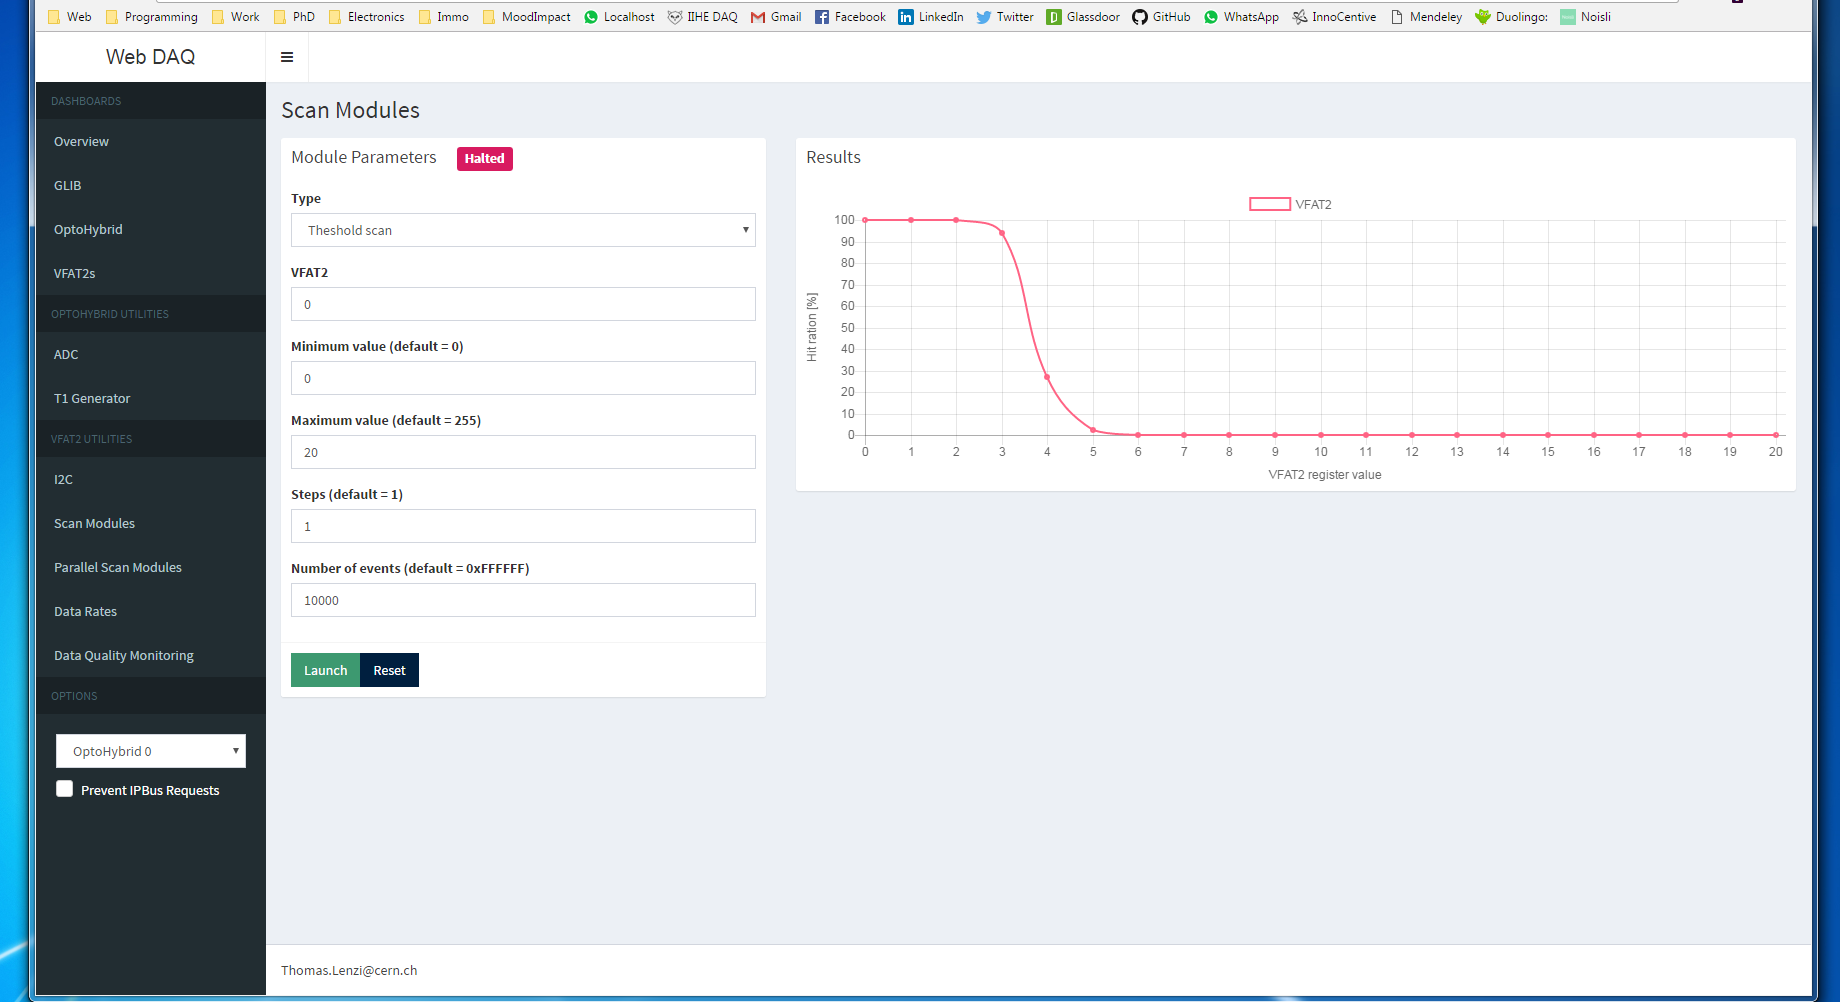
\includegraphics[width=\textwidth]{img/II-3-test-beam/app-scan.png}
        \caption{???}
        \label{fig:II-3-app-calibration}
      \end{figure}

    \subsection{Data Quality Monitoring}

      Data Quality Monitoring (DQM) is used online to check the consistancy of data recorded. This is the last component of the application shown in Figure \ref{fig:II-3-app-tk}. This page monitors the status of the readout buffers of the GLIB and allows the user to acquire data. Once acquisition has started, plots begin to fill with the various parameters extracted from the VFAT2 data format. The user can visualise the number of data packets, the BC, EC, flags, and chip ID distribution, the occupancy of the strips, etc. The user can monitor the validity of the data and if required change the parameters of the run. Although this application has the ability to readout data and store it to disk, it was not used to this intend during the test beam. A XDAQ based program developped by the software development team of the GEM collaboration was used to acquire raw data from the GLIB and store it on disk in text files for later analysis.

      \begin{figure}[h!]
        \centering
        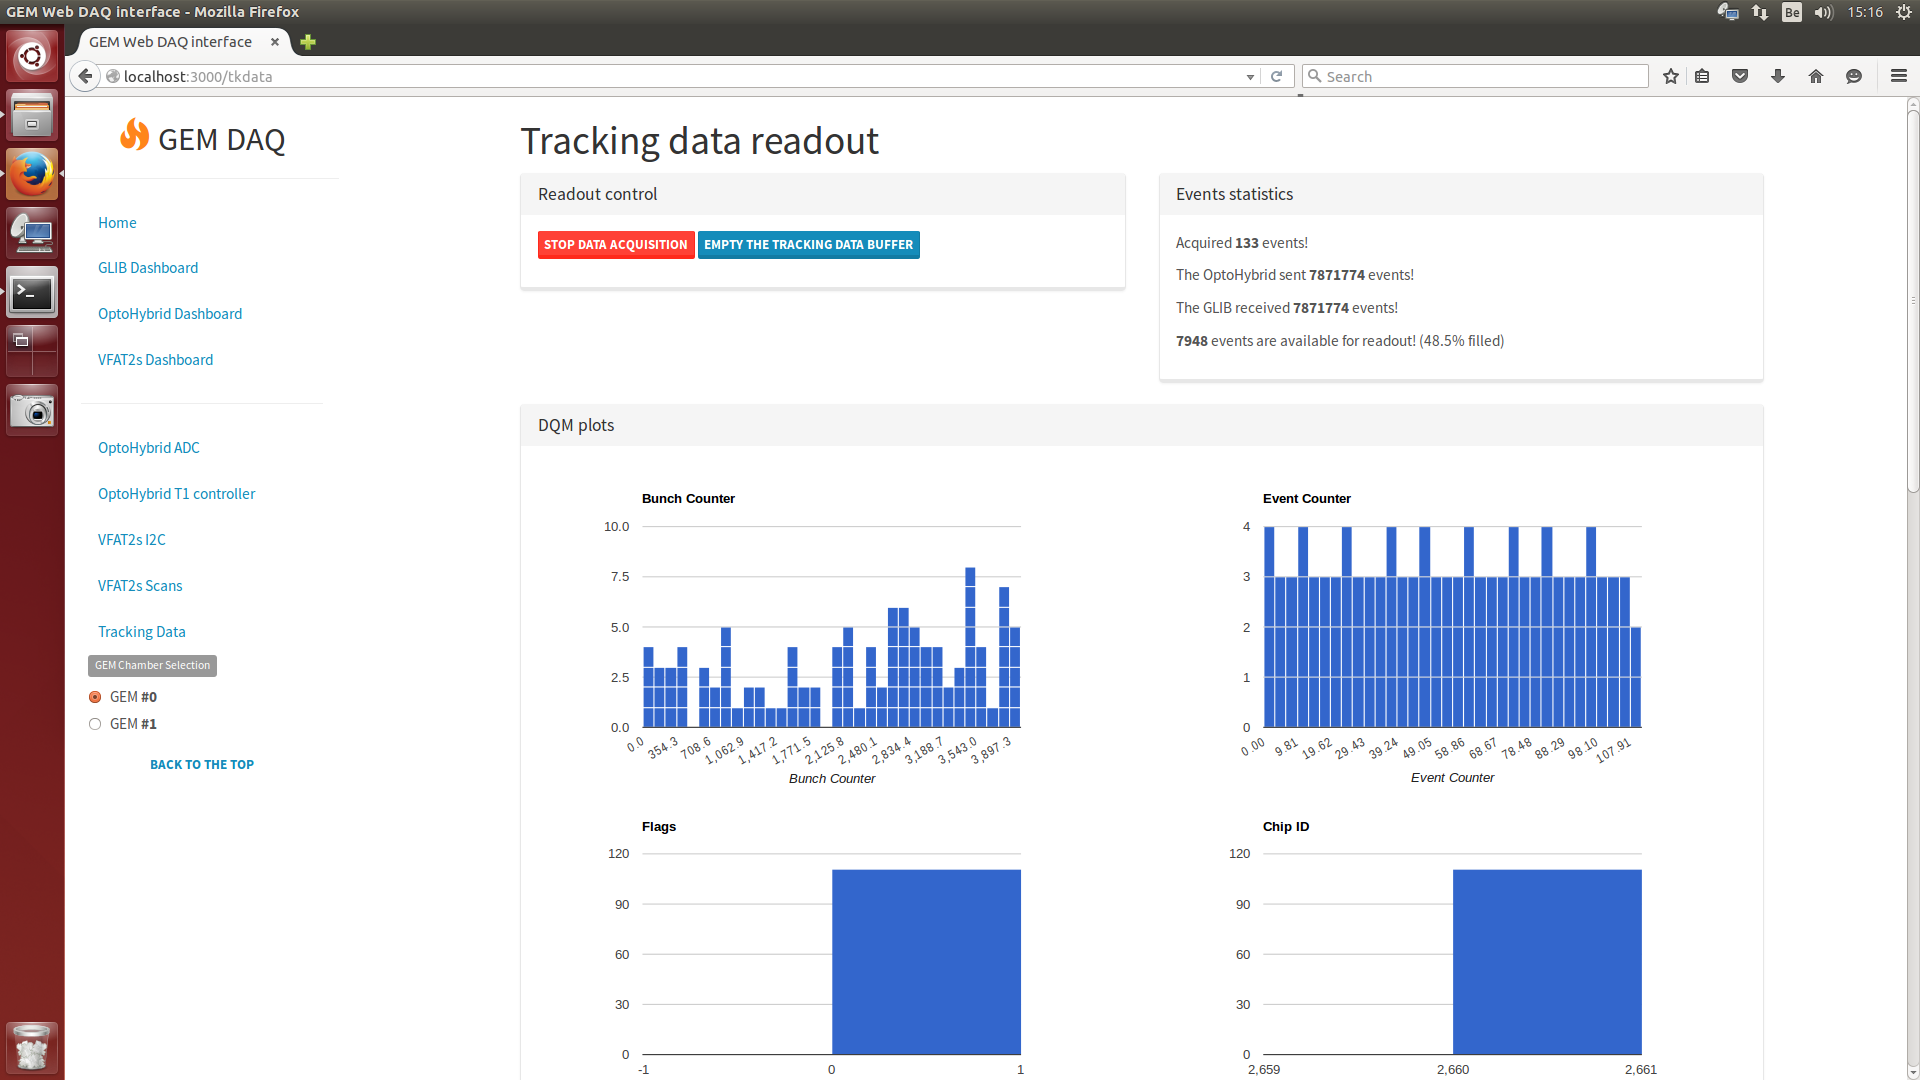
\includegraphics[width=\textwidth]{img/II-3-test-beam/app-tk.png}
        \caption{???}
        \label{fig:II-3-app-tk}
      \end{figure}

  \section{The Test Beam Setup}

    The test beam campaigns take place at CERN in the North Area of Prevessin, one of the secondary sites. The beam provided to the experiments originates from the SPS proton bunches which are extracted from the accellerator at 400 GeV and interact with four primary targets (T2, T4, T6, and T10) to produce the secondary beams mainly composed of electrons and hadrons. A selection on the type of particles and their momentum is performed and the beam is guided towards the experimental setups, namelly H2 and H4, using dipole magnets. In the transfer tunnels, collimators can be adjusted to increase or reduce the flux of particles and an optionnal secondary target can be placed in the beam path to create a tertiary beam. Figure \ref{fig:II-3-sps} shows the monitoring page of the SPS indicating the presence of spills of particles in yellow. Spills last between 4.8 s and 9.6 s and repeat every 14 s to 48 s depending on the SPS operation. \\

    \begin{figure}[h!]
      \centering
      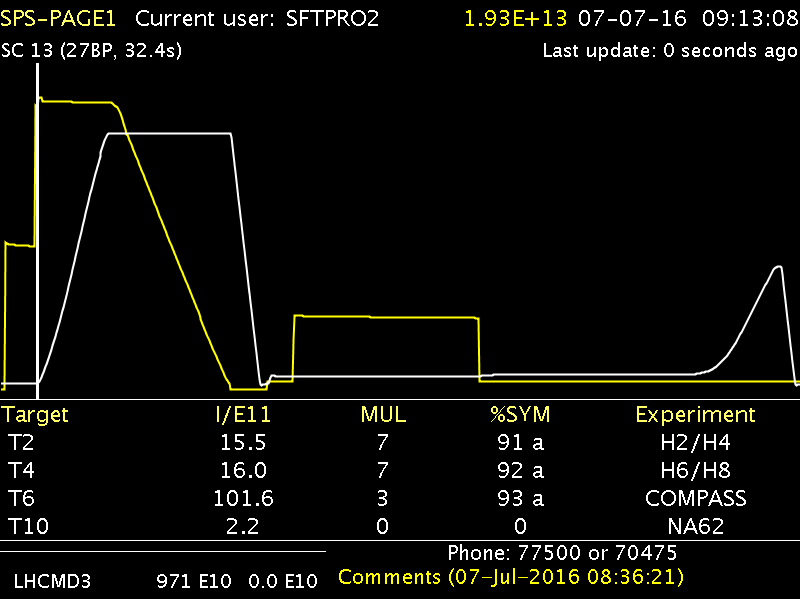
\includegraphics[width=0.8\textwidth]{img/II-3-test-beam/sps.png}
      \caption{???}
      \label{fig:II-3-sps}
    \end{figure}

    The two types of particles used during the test beam were pions and muons. Pions are obtained from the secondary beam by inserting a thin absorber which removes the electronic component of the beam. They can reach intensies between 10$^4$ and 10$^7$ particles per spill and produce a very narrow beam. From their decay, a muon beam can be obtained by using moderate intensity secondary beams and closing the collimators. The muon beam reaching the experimental setup is a wider and less intense.

    \subsection{The GEM Detectors Setup}

      During the November 2015 test beam campaign, a superchamber of GE1/1-V detectors has been used to collect data. Each detector was equipped with 12 VFAT2 Hybrids mounted in the central four rows. The remaining slots, too far away from the beam spot, were been covered with grounding equipement to reduce noise. Each GEM was mounted with a GEB v2 and a OptoHybrid v2a. A picture of the setup is represented in Figure \ref{fig:II-3-test-geb}. Both OptoHybrids were connected to the same GLIB placed in a microTCA crate. \\

      \begin{figure}[p!]
        \centering
        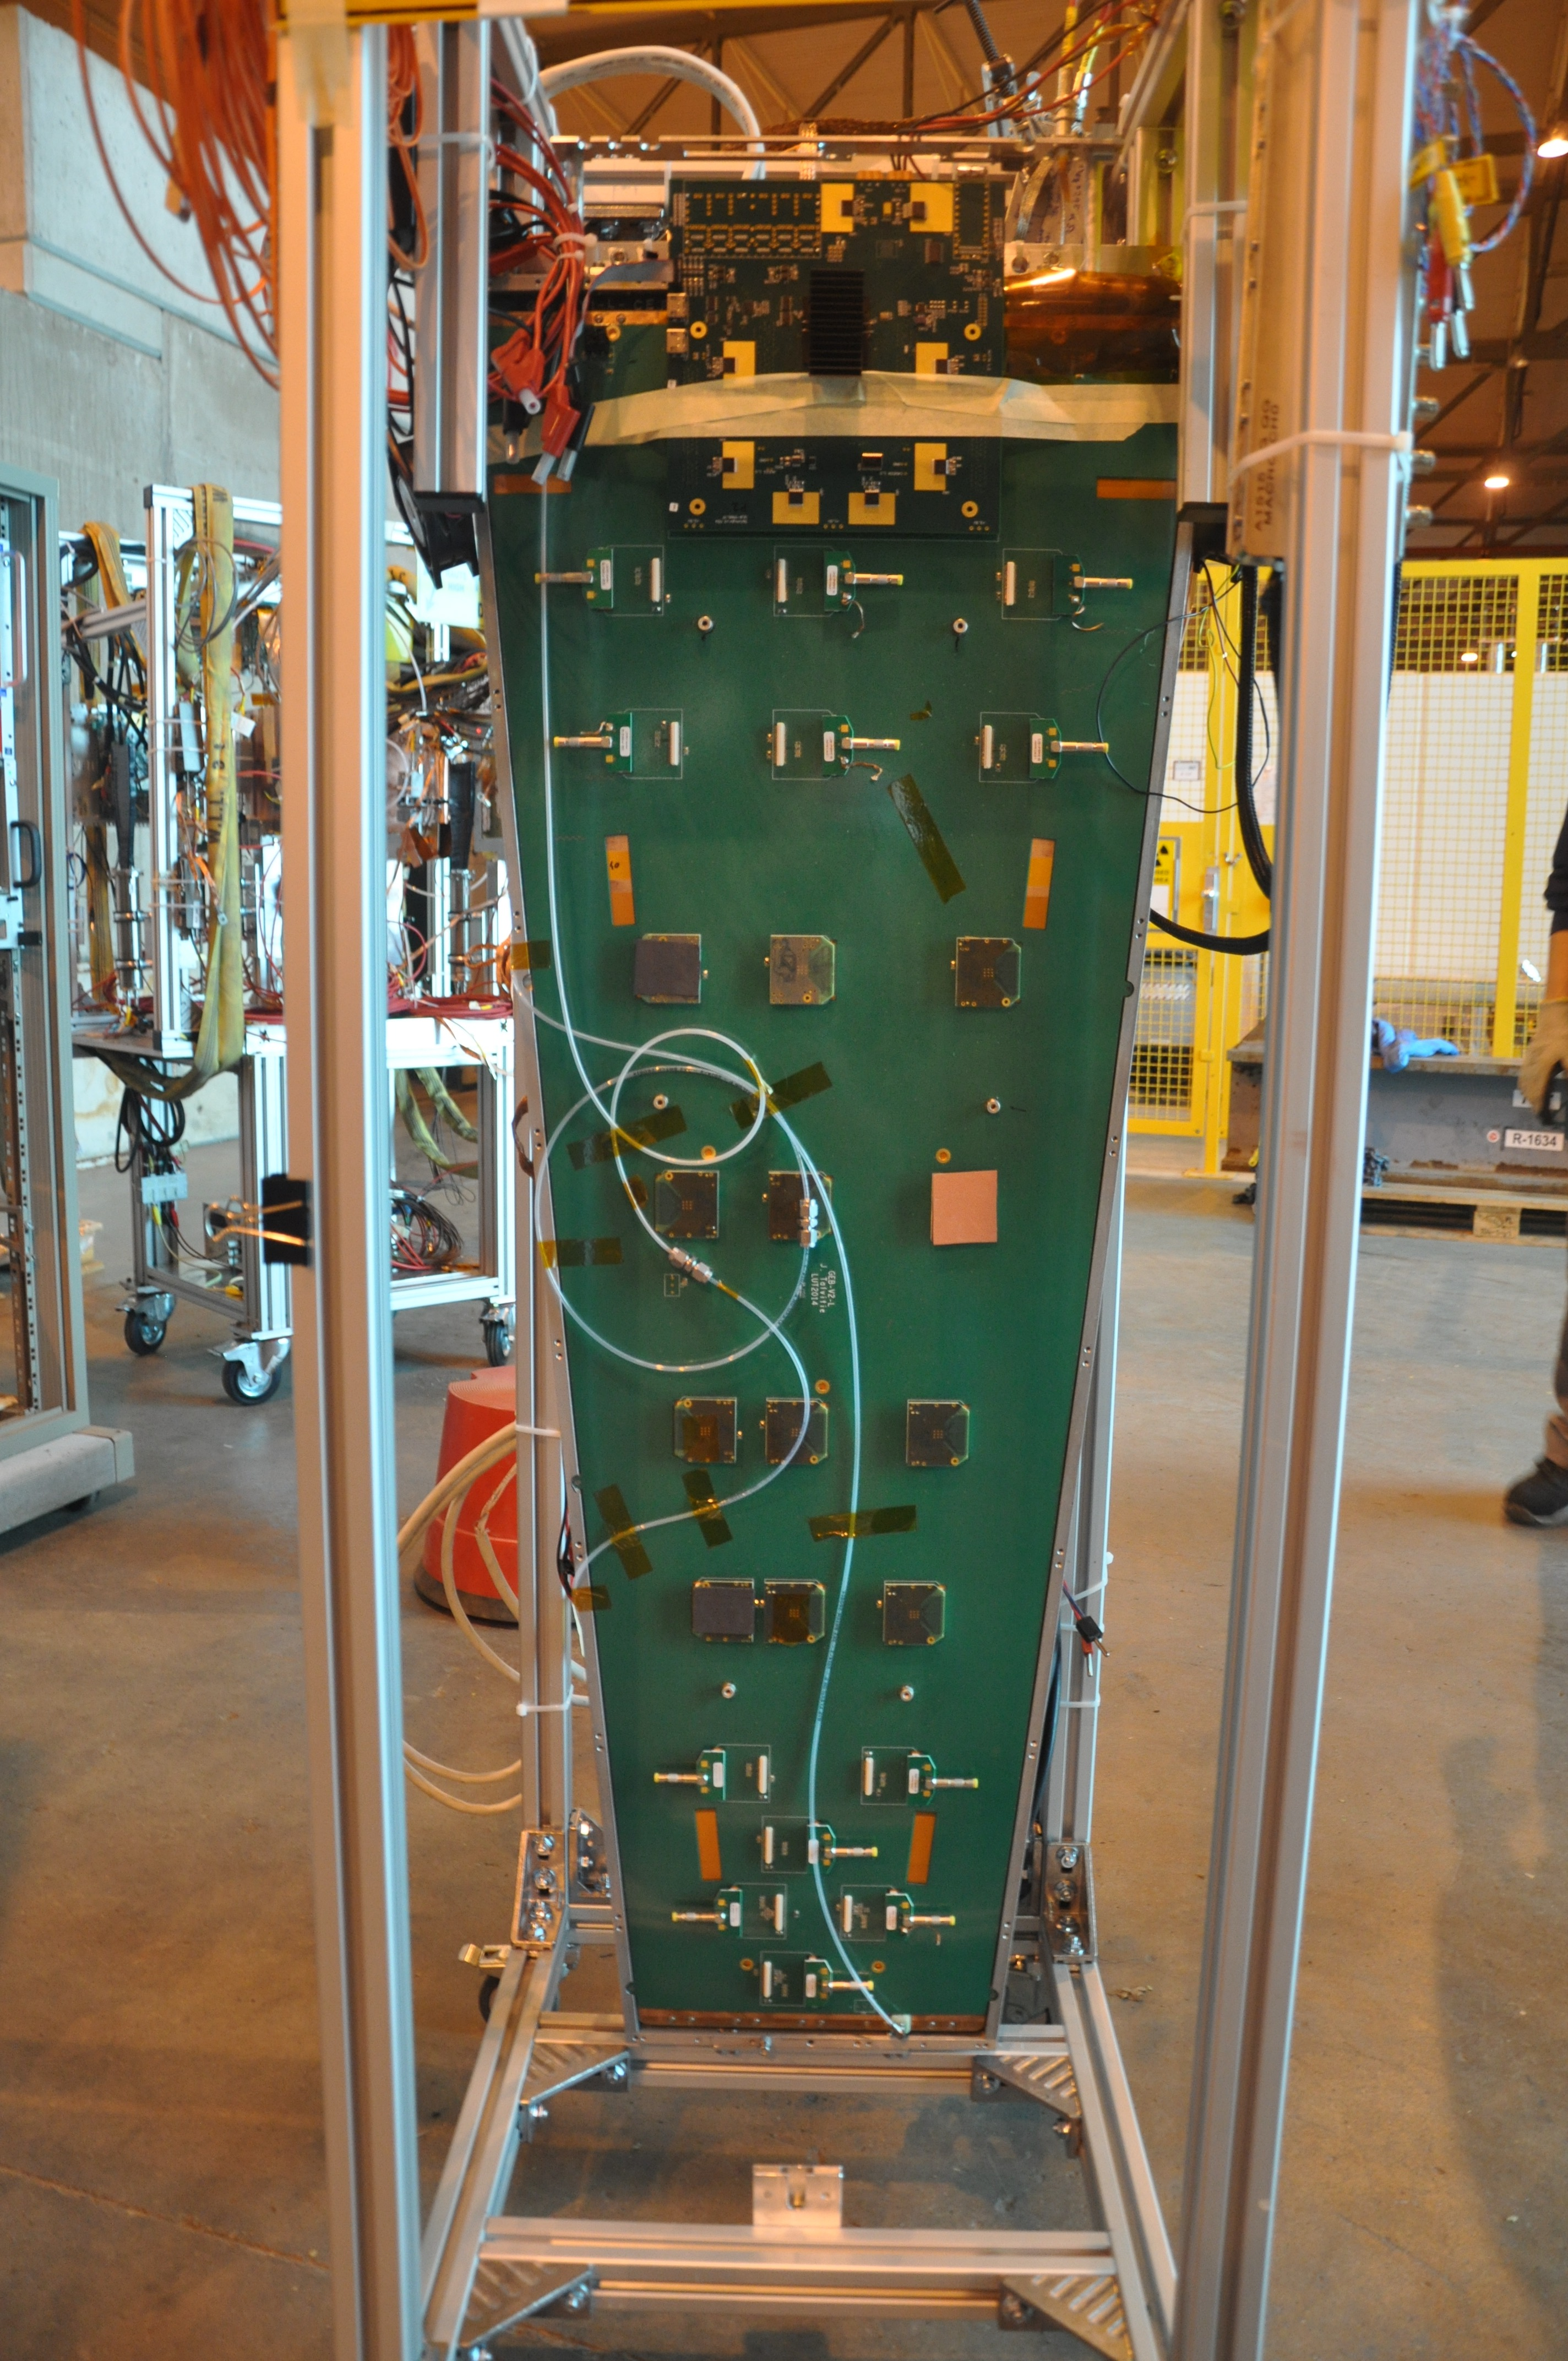
\includegraphics[width=\textwidth]{img/II-3-test-beam/test-geb.jpg}
        \caption{???}
        \label{fig:II-3-test-geb}
      \end{figure}

      The GEM detectors were connected to a gas system providing a mixture of Ar/CO$_2$ at 70\% and 30\% respectivly. The high-voltage was delivered through a ceramic high-voltage divider for one chamber and by separate channels connected directly to the GEM foils and planes for the other. The high-voltage applied is expressed in terms of current flowing through the divider which, by suming up the individual resistors that it is made of, yields a value in volts. Table \ref{tab:II-3-test-hv} enumarates the different values of the voltages according to the current flowing through the divider. The difference between the divider and drift plane values is due to an input filter placed before the latter which smoothes out fluctuations in the voltage. The low voltages for the OptoHybrids (1.8 V and 4 V) and for the GEBs (2.5 V) were delivered by two power boards mounted on top of the detector stand along with the necessary tools to reprogram the FPGA in case of failure and the debugging headers.

      \begin{table}[h!]
        { \footnotesize
        \begin{tabularx}{\textwidth}{|C{1}|C{1}|C{1}|C{1}|C{1}|C{1}|C{1}|C{1}|C{1}|}
          \hline \textbf{Current ($\mu$A)} & \textbf{Divider (V)} & \textbf{Drift plane (V)} & \textbf{GEM1 top (V)} & \textbf{GEM1 bottom (V)} & \textbf{GEM2 top (V)} & \textbf{GEM2 bottom (V)} & \textbf{GEM3 top (V)} & \textbf{GEM3 bottom (V)} \\ \hline
          700 & 3921 & 3290 & 2503 & 2107 & 1801 & 1416 & 805 & 437 \\
          710 & 3977 & 3337 & 2538 & 2137 & 1827 & 1437 & 816 & 443 \\
          720 & 4033 & 3384 & 2574 & 2167 & 1853 & 1457 & 828 & 450 \\
          730 & 4089 & 3431 & 2610 & 2198 & 1879 & 1477 & 839 & 456 \\
          740 & 4145 & 3478 & 2646 & 2228 & 1904 & 1497 & 851 & 462 \\
          750 & 4201 & 3525 & 2682 & 2258 & 1930 & 1518 & 862 & 468  \\
          760 & 4257 & 3572 & 2717 & 2288 & 1956 & 1538 & 874 & 475 \\
          770 & 4313 & 3619 & 2753 & 2318 & 1981 & 1558 & 885 & 481 \\
          780 & 4369 & 3666 & 2789 & 2348 & 2007 & 1578 & 897 & 487 \\
          790 & 4425 & 3713 & 2825 & 2378 & 2033 & 1598 & 908 & 493 \\
          800 & 4481 & 3760 & 2860 & 2408 & 2059 & 1619 & 820 & 500 \\
          810 & 4537 & 3807 & 2896 & 2438 & 2084 & 1639 & 931 & 506 \\ \hline
        \end{tabularx}
        }
        \caption{??}
        \label{tab:II-3-test-hv}
      \end{table}

    \subsection{The Beam Area Setup}

      The GE1/1 superchamber has been inserted in the beam path and adjusted so that solely one VFAT2 in the middle column would be exposed to the beam spot. Figure \ref{fig:II-3-test-setup} shows the setup on the left placed in front of the beam transfer tunnel on the right side. Four scintillators, three placed in front of the detector and visible in the picture, and one placed in the back of the detector were used to provide triggers to the system. The output of the four scintillators was converted to Nuclear Instrumentation Module (NIM) logic and their coincidance used as the trigger source of the system. \\

      \begin{sidewaysfigure}[p!]
        \centering
        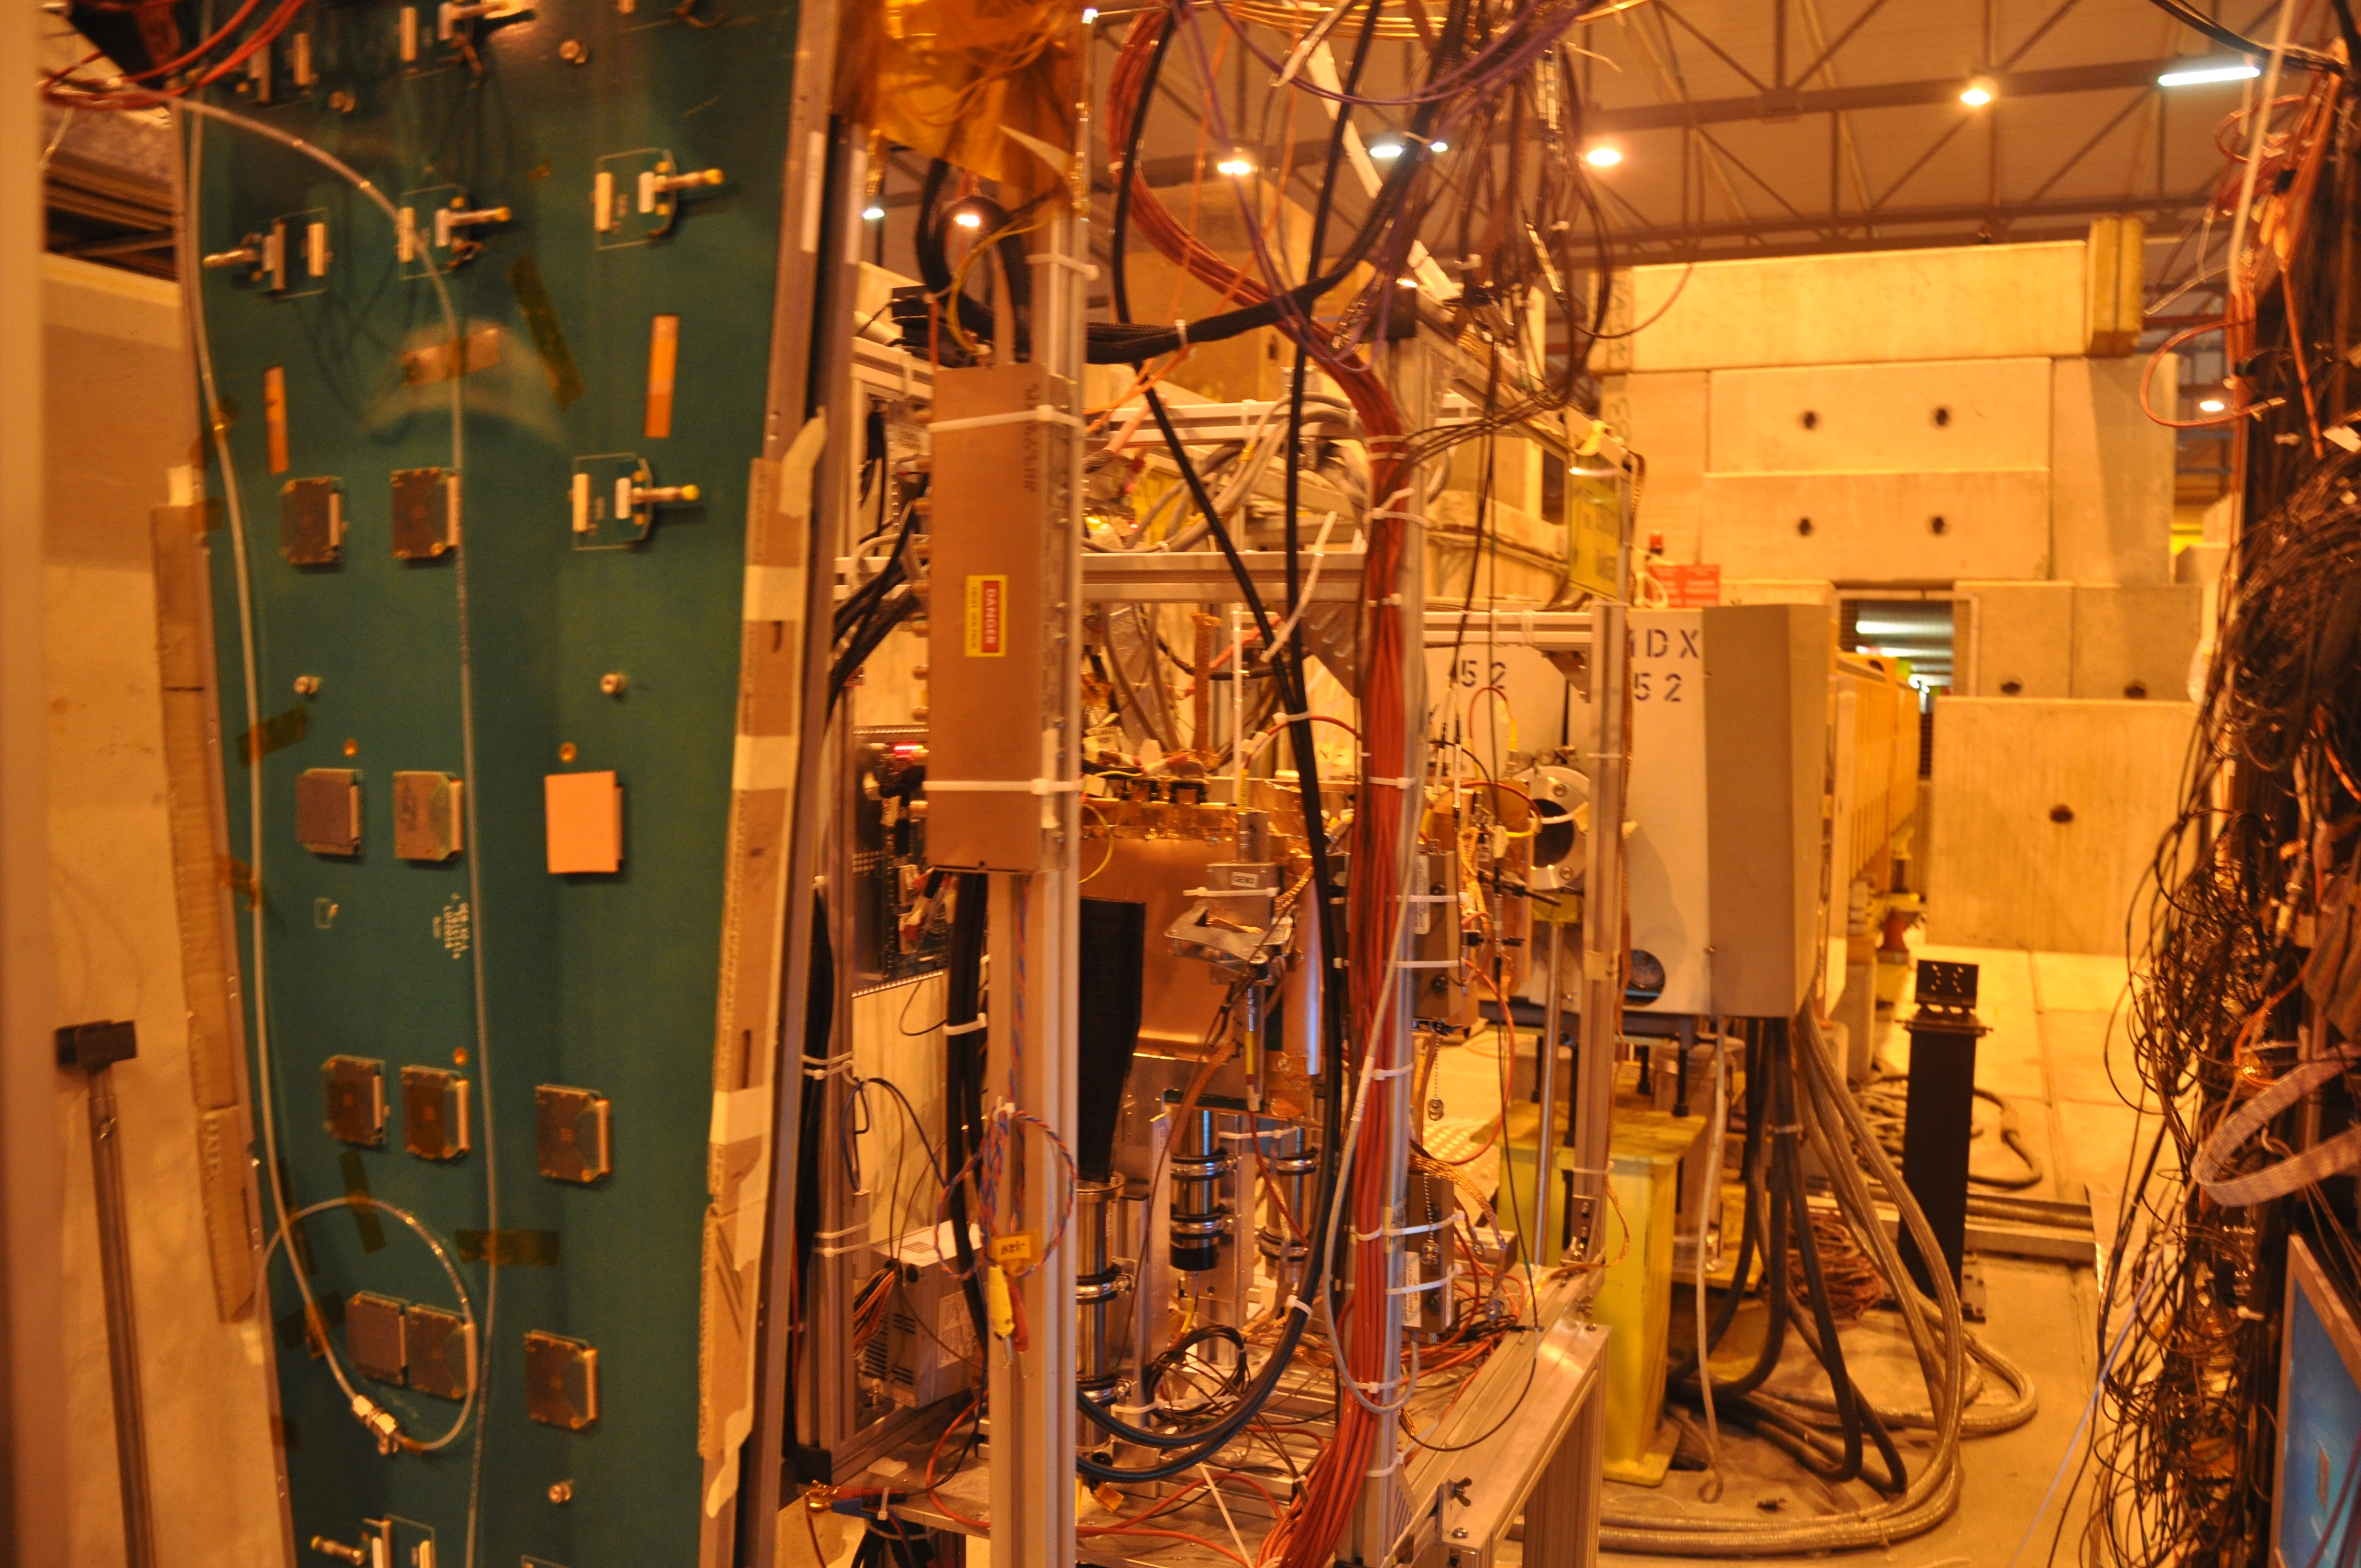
\includegraphics[width=0.9\textwidth]{img/II-3-test-beam/test-setup.jpg}
        \caption{???}
        \label{fig:II-3-test-setup}
      \end{sidewaysfigure}

      NIM uses current driven logic levels which produce -0.8 V over 50 $\Omega$ for a logic '1' and 0 V for a logic '0'. As the OptoHybrids use TTL voltage driven levels, namelly 2.5 V for a logic '1' and 0 V for a logic '0', a converter had to be used. It was observed that the output levels of the NIM to TTL module were close to the switching voltage and might affect the number of triggers seen by the OptoHybrids. It was computed that this situation occured in less than 1/10 000 events and could be solved by the offline analysis. Checks were performed to ensure the source of the problem did not originate from the DAQ system itself, which was proven not to be the case.

  \section{Data Analysis}

    The data collected during the test beam was analysied to study the detector performance according to various parameters. Data was taken at multiple high-voltage values, VFAT2 threshold settings, and particle rates. An analysis framework has been developped in order to combine the readout data from the two GE1/1 chambers. Aligment of the events was non-trivial and based on the difference between two consecutive BC values of the events. Indeed, due to the problem exposed hereabove with the trigger logic and the fact that the two VFAT2s are not garanteed to have the same value of the BC counter at the same time, matching of the events based on the absolute value of the BC could not be done. Therefore, the difference between the BCs of two consecutive events in the data stream was computed and matched between the two datasets. When a discrepancy arose, one of the datasets had to be realigned. Once realigment was performed, analysis tools had access to both chambers for each event.

    \subsection{VFAT2 Threshold Scans}

      The first parameter to study is the noise on the VFAT2s induced by the system and by the antena effect of the strips. To this end, threshold scans have been produced using the web application. These scans are ran when the beam is not present. They use the trigger bits of the VFAT2s which do not need a L1A source to be produced. They are sampled at 40 MHz and for each threshold value the ratio of events containing hits against the total amount of collected events is defined to be the noise. Figure \ref{fig:II-3-data-threshold} plots the noise level as a function of the VFAT2 threshold in terms of VFAT2 units, the decimal value written in the 8 bit register afterwards converted to a voltage level, for GEM0 on the left and GEM1 on the right with muons. Although the noise level quickly diminishes, it never reaches the expected value of 0 even at very high threshold. Typically, previous test beams have shown that a value of 15 kills the noise. Furthermore, it can be seen that noise level is higher in GEM1, which reaches 20\% at a threshold value of 10 against 15\% for GEM0. From the threshold scans, it was decided to run both chambers at a VFAT2 threshold level of 25 for data taking runs. This value is considered to be the default threshold except if otherwise specified. \\

      \begin{figure}[h!]
        \centering
        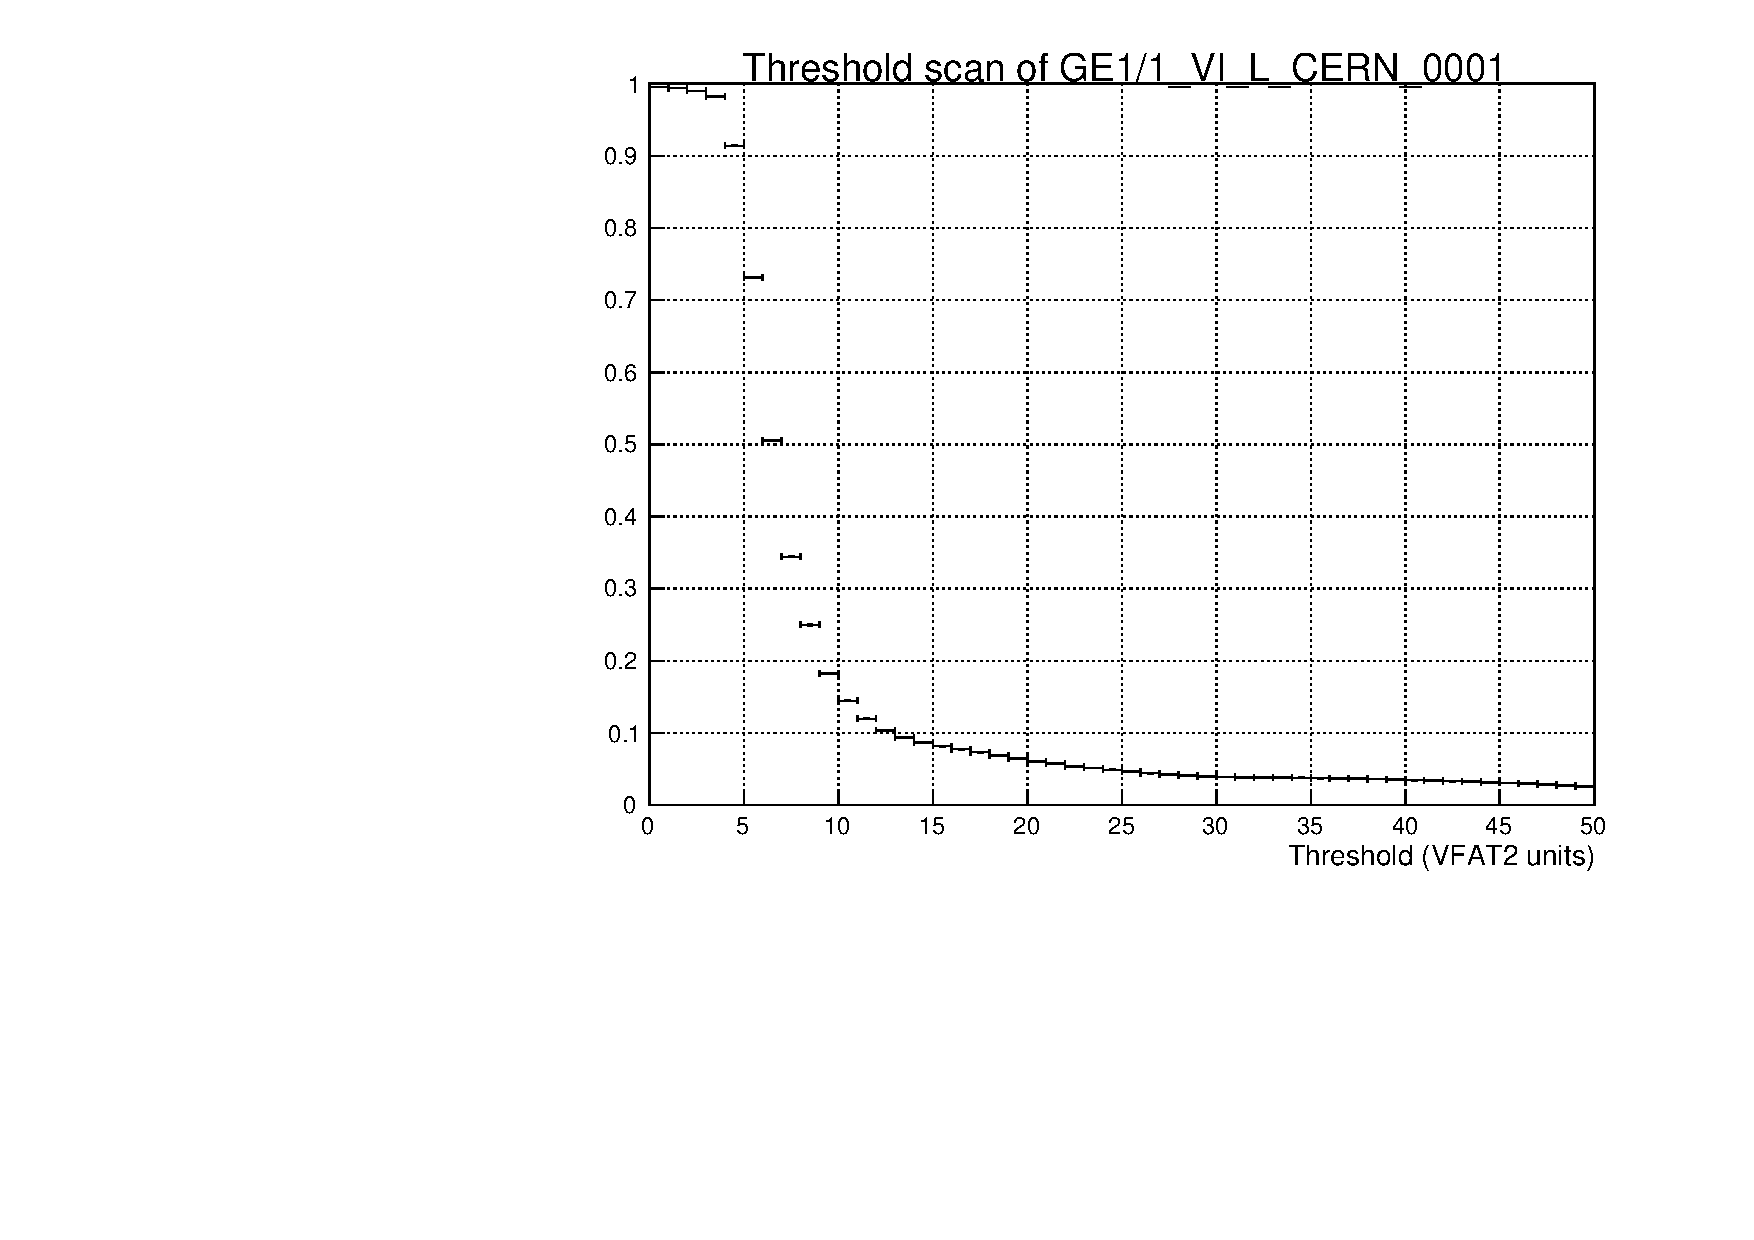
\includegraphics[width=0.49\textwidth]{img/plots/cThresholdScan_GEM0}
        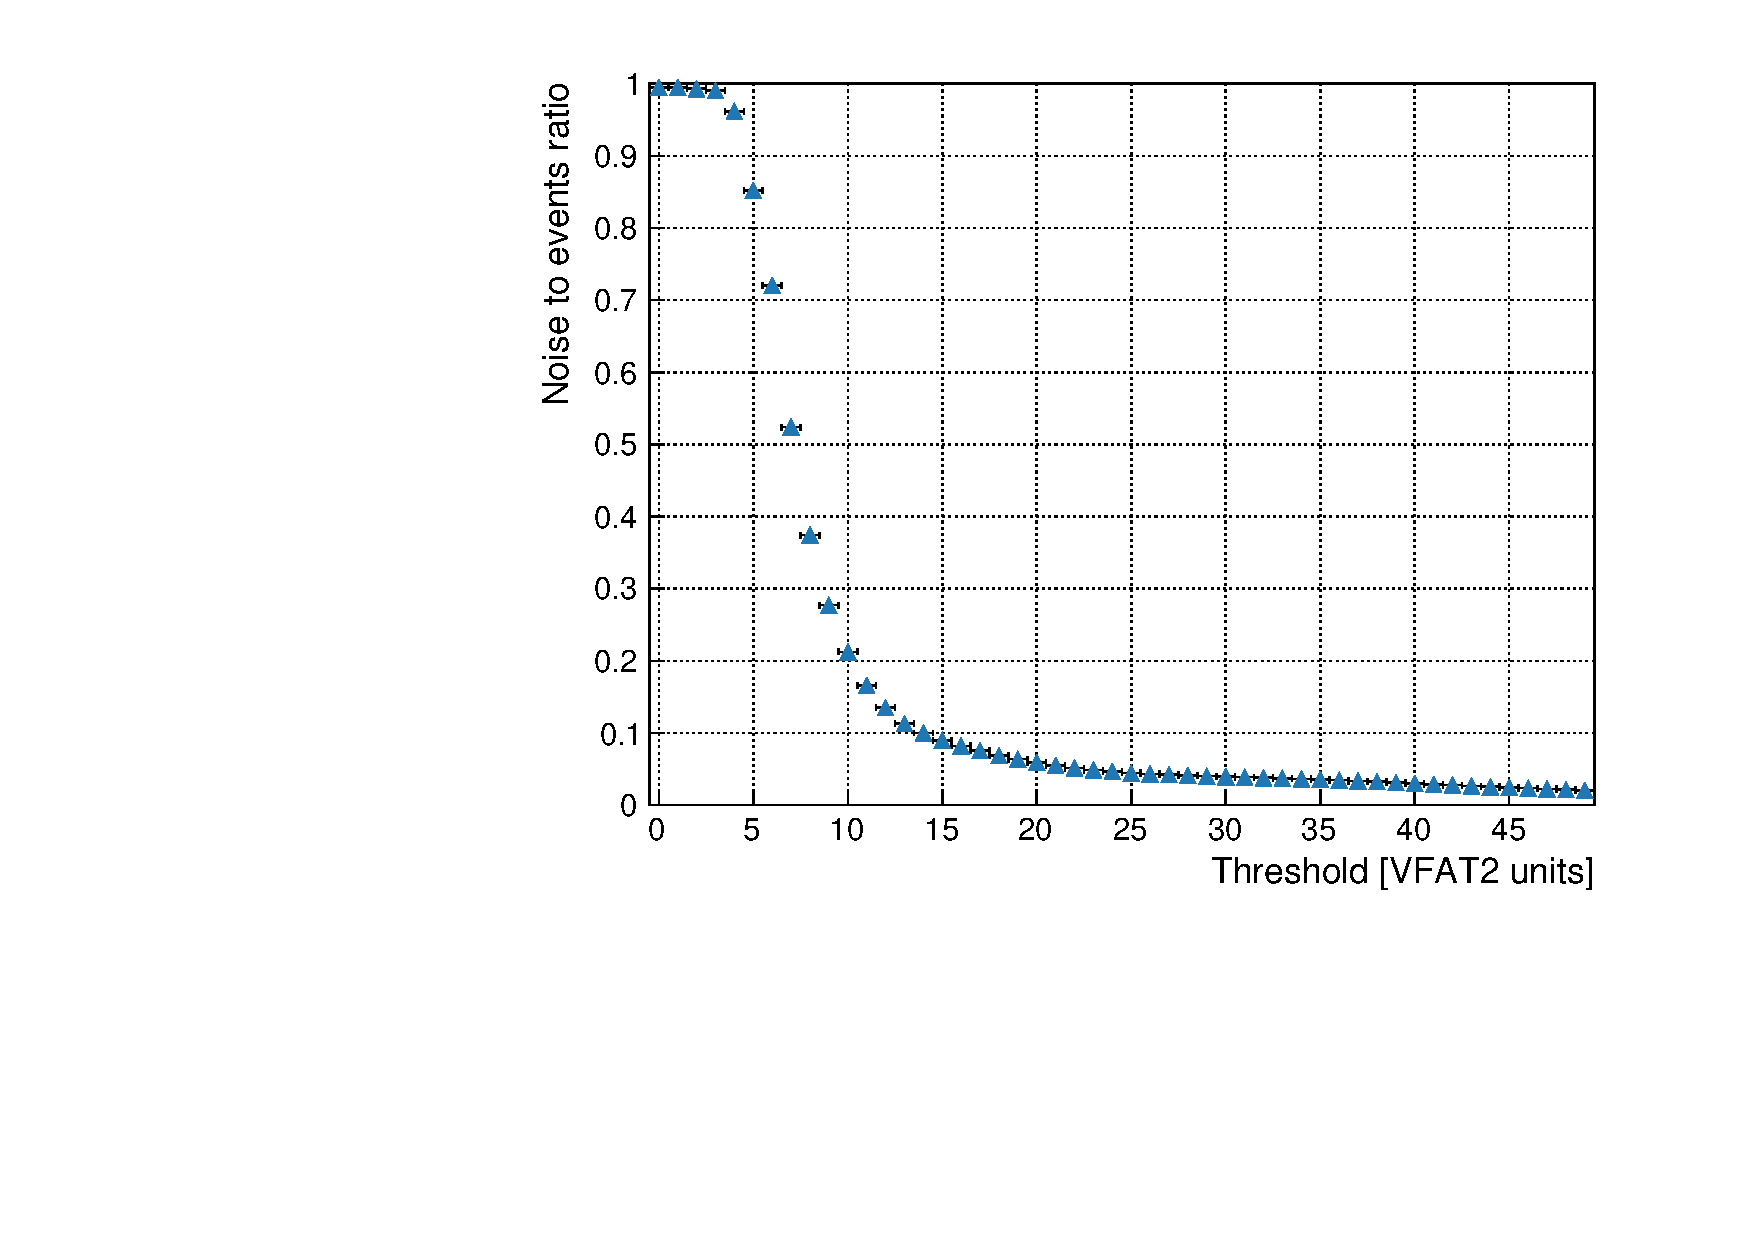
\includegraphics[width=0.49\textwidth]{img/plots/cThresholdScan_GEM1}
        \caption{Plots of the noise level as a function of the VFAT2 threshold in terms of VFAT2 units, the decimal value written in the 8 bit register afterwards converted to a voltage level, for GEM0 on the left and GEM1 on the right with muons.}
        \label{fig:II-3-data-threshold}
      \end{figure}

      After the end of the test beam, the noise issue has been investigated toroughlty and two sources have been isolated: the I2C clock used for the slow communication and the LEMO cables used for the trigger input. In the version of the firmware used during the test beam, the I2C clock runs continuously which induces noise on the trigger bits of the VFAT2s at a frequency of 100 kHz, the same as the clock itself. This problem has been solved by activating the I2C clock solely when a slow control operation takes place, limiting the number of corrupted trigger bits. The second issue originated from current loops formed between the low power cables of the OptoHybrids and the LEMO cable connecting the system to the NIM crate. The ground of the latter was connected to the OptoHybrid ground through the shielding of the LEMO cables. Once the two ground systems were isolated, noise level comparable to previous observations were obtained. \\

      It was also observed that GEM1 experienced a leakage current through the GEM foils of about 10 $\mu$A. This had as consequence to reduce the voltage on the GEM foils and thus decrease the gain and efficiency of the detector. The detector also suffered from water condensation inside the gas pipes which caused some problems during the first days of run. These issues can explain the difference in noise observed between the two chambers.

    \subsection{VFAT2 Latency Scans}

      Once the threshold on the VFAT2s has been set and the beam has been turned on, a latency scan has to be done in order to capture the events corresponding to the triggers coming from the scintillators. Again the web application is used to run the scan on the VFAT2s. Similarly to the threshold scan, the latency scan counts the ration of events with a hit against the total number of events. However, it uses the tracking data provided by the VFAT2s and not the trigger bits. Figure \ref{fig:II-3-data-latency} plots the ratio of hit events as a function of the VFAT2 latency in terms of BXs for a monostable pulse length of four clock cycles for GEM0 on the left and GEM1 on the right with muons. When the latency is too low or too high, the VFAT2 misses the hit and a baseline value of 0.05 is observed corresponding to noise. Once the latency enters the correct windows, it rises to a value close to 0.98. This plot illustrates the usefullness of the settable monostable pulse length. Indeed, the two points at approximatly 0.5 and 0.6 indicate that hits are falling in two adjacent latency values, each collecting half the events. In case of a non-adjustable setting, the maximum efficiency of the system would be reduced by half. From these results, a VFAT2 latency value of 11 has been used for data taking runs. This value is considered to be the default latency except if otherwise specified. \\

      \begin{figure}[h!]
        \centering
        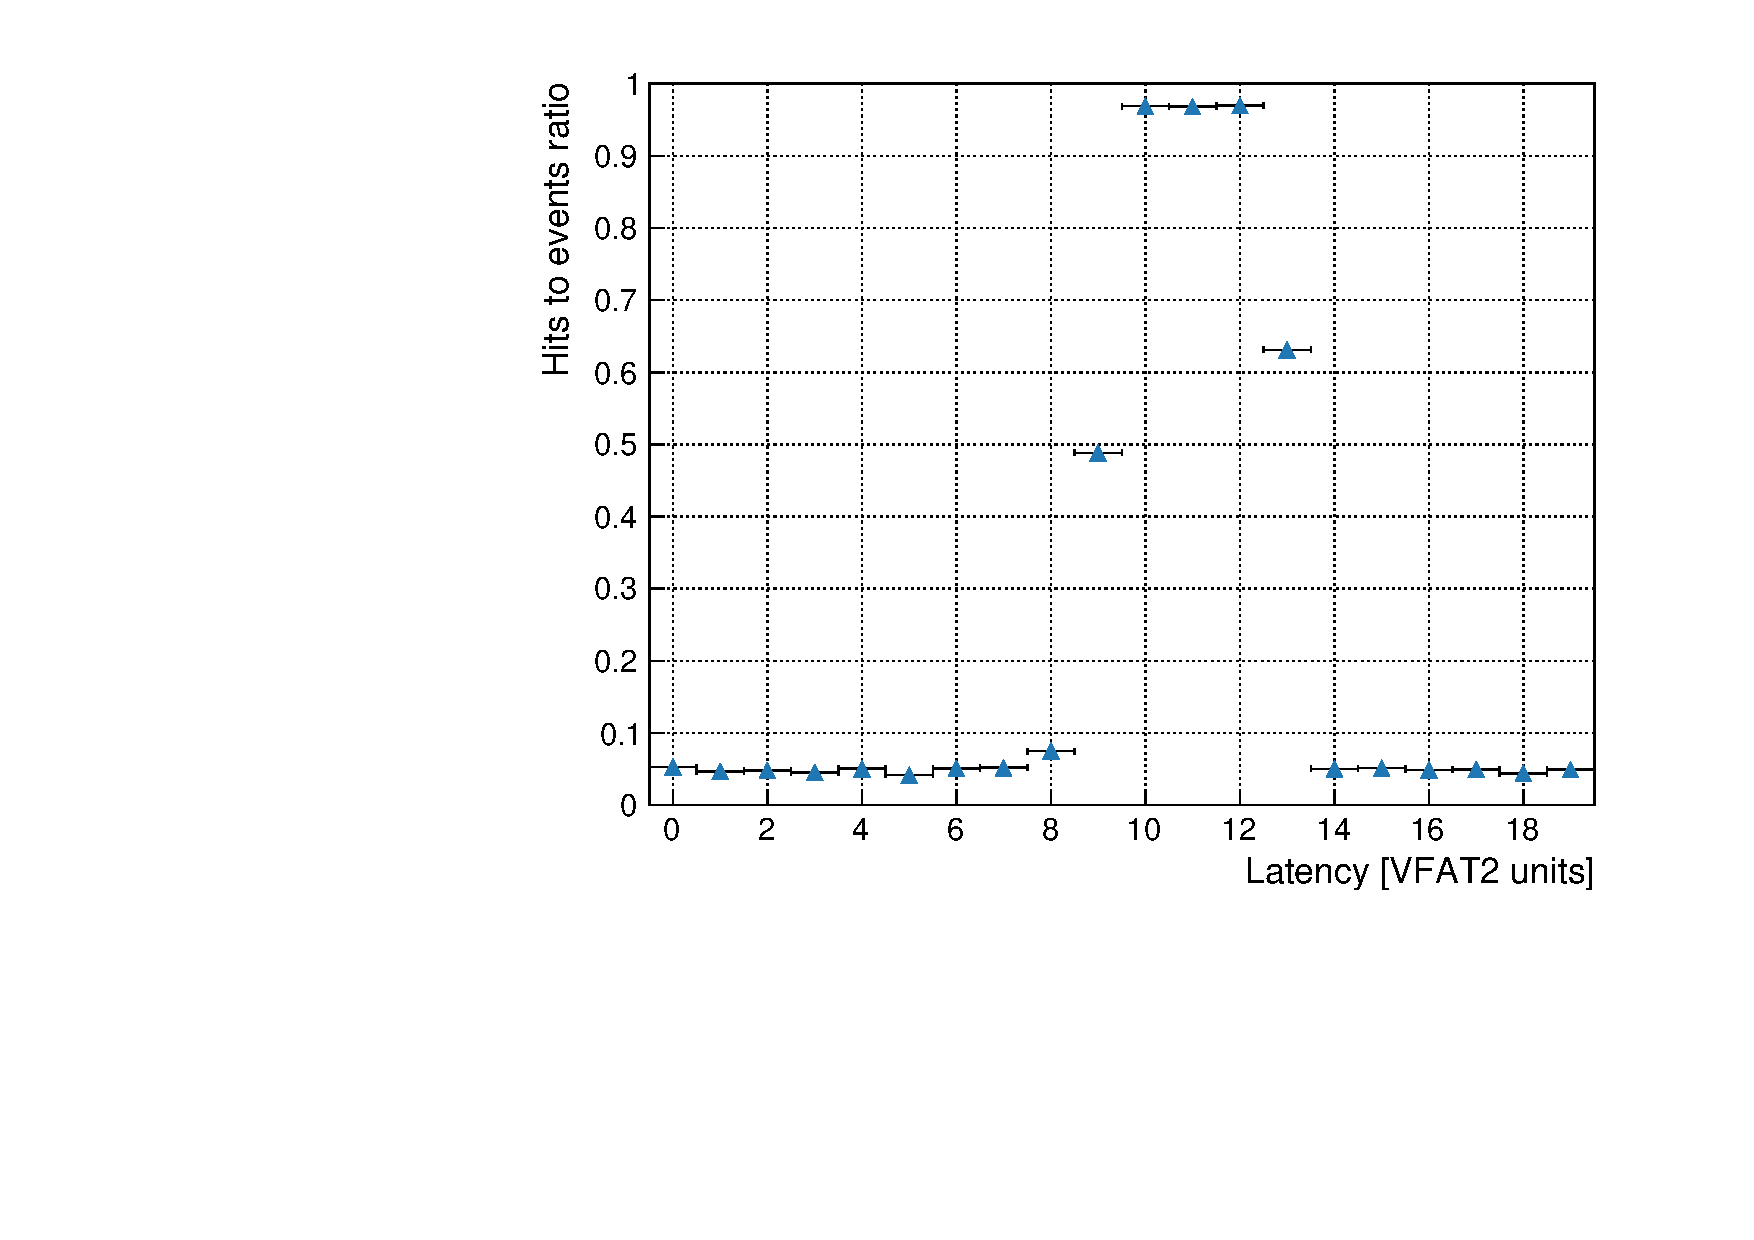
\includegraphics[width=0.49\textwidth]{img/plots/cLatency_GEM0}
        
\includegraphics[width=0.49\textwidth]{img/empty.png}
        \caption{Plots of the ratio of hit events as a function of the VFAT2 latency in terms of BXs for a monostable pulse length of four clock cycles for GEM0 on the left and GEM1 on the right with muons.}
        \label{fig:II-3-data-latency}
      \end{figure}

      Latency scan are also used to measure the noise and the efficiency of the detector. When looking at out-of-time events, the only contribution to the hits is noise. On the other hand, when considering the window in which the latency is well adjusted, both the noise and the particle hits play a role in the measurment. Taking this value to be the measured efficiency, it corresponds to the ratio between the number of events detected by the GEM detector and those detected by the scintillator system. However, the measured efficiency is the superposition of two poisson processes: the noise and the real detector efficiency. In order to obtain the computed or real efficieny, simulations were developped to compute upper and lower limits on the real efficiency according to the noise levels. This was achived by running a thousand pseudo-experiments for each possible efficiency value and comparing the result to the measured value. With a noise level of 100\%, the real efficiency could be anything between 0\% and 100\%. However, with a noise level of 1\%, the computed efficiency will be close to the measured efficiency.

    \subsection{Efficiency against High-Voltage}

      Using the latency scan to compute noise and efficiency values, the evolution of these parameters has been studied according to the high-voltage applied on the detector. Figure \ref{fig:II-3-data-eff-hv} plots the measured noise (green), measured efficiency (blue), and computed efficiency (orange) as a function of the high-voltage expressed in $\mu$A for GEM0 on the left and GEM1 on the right with muons. Both results show an increase in efficiency with the high-voltage, reaching a plateau around 98\%. This is caused by the higher gain at which the GEM foils start to operate which in turn amplifies the signals and allows for it to be detected by the VFAT2 ASIC. It can be noted that a shift exists between the results for GEM0 and GEM1. Values for the latter are shift to the left by approximatly 10 $\mu$A. While GEM0 reaches a plateau at 800 $\mu$A, GEM1 requires 810 $\mu$A to reach an efficiency around 98\%. This is due to the leakage current observed during installation which decreases the voltage applied to the GEM foils and in turn performance. It can also be noted that the noise is constant with the high-voltage. These results were compared against previous test beam campaign results \cite{KARCHIN2012561} and are in excellent accordance with each other. From this, it was decided to operate both chambers at 800 $\mu$A as sparks were sometimes observed at 810 $\mu$A. This value is considered to be the default high-voltage except if otherwise specified.

      \begin{figure}[h!]
        \centering
        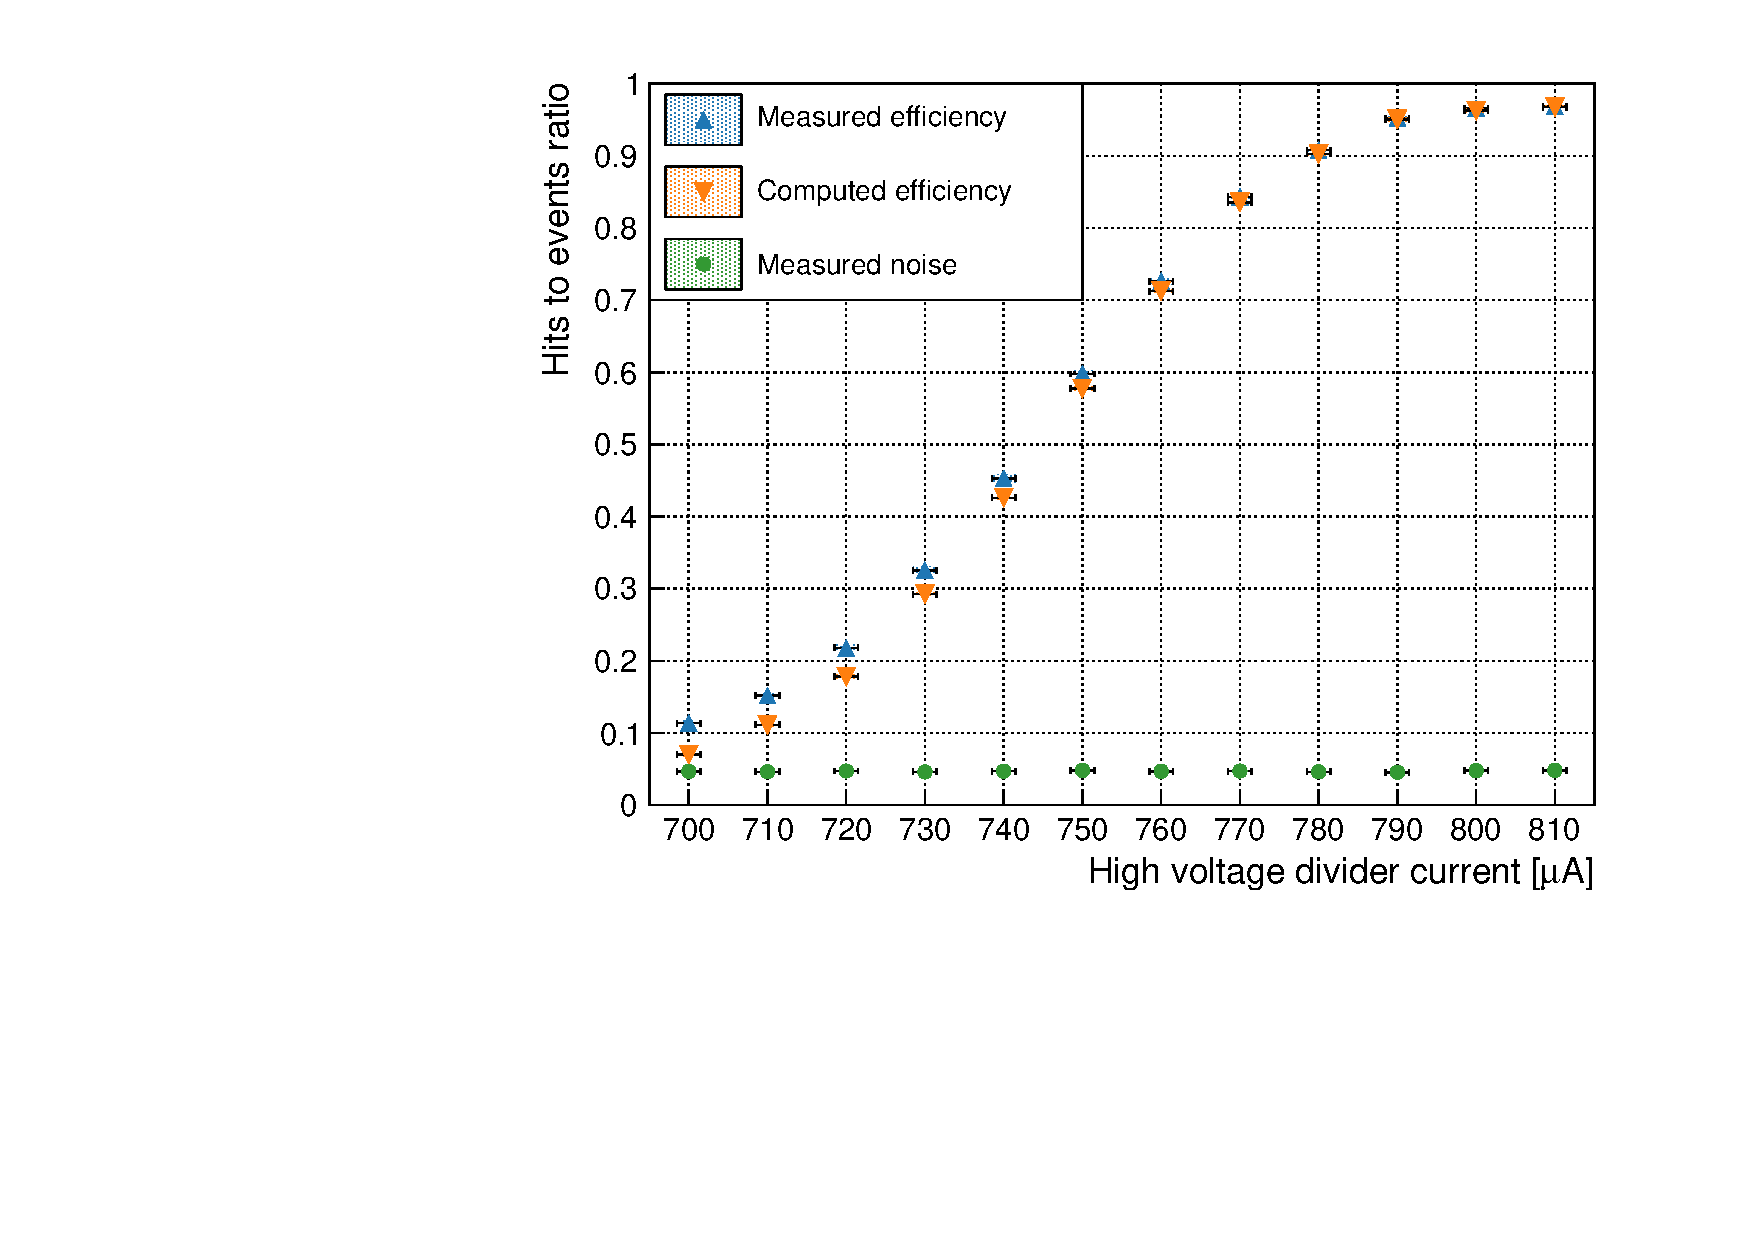
\includegraphics[width=0.49\textwidth]{img/plots/cEfficiency_HV_GEM0}
        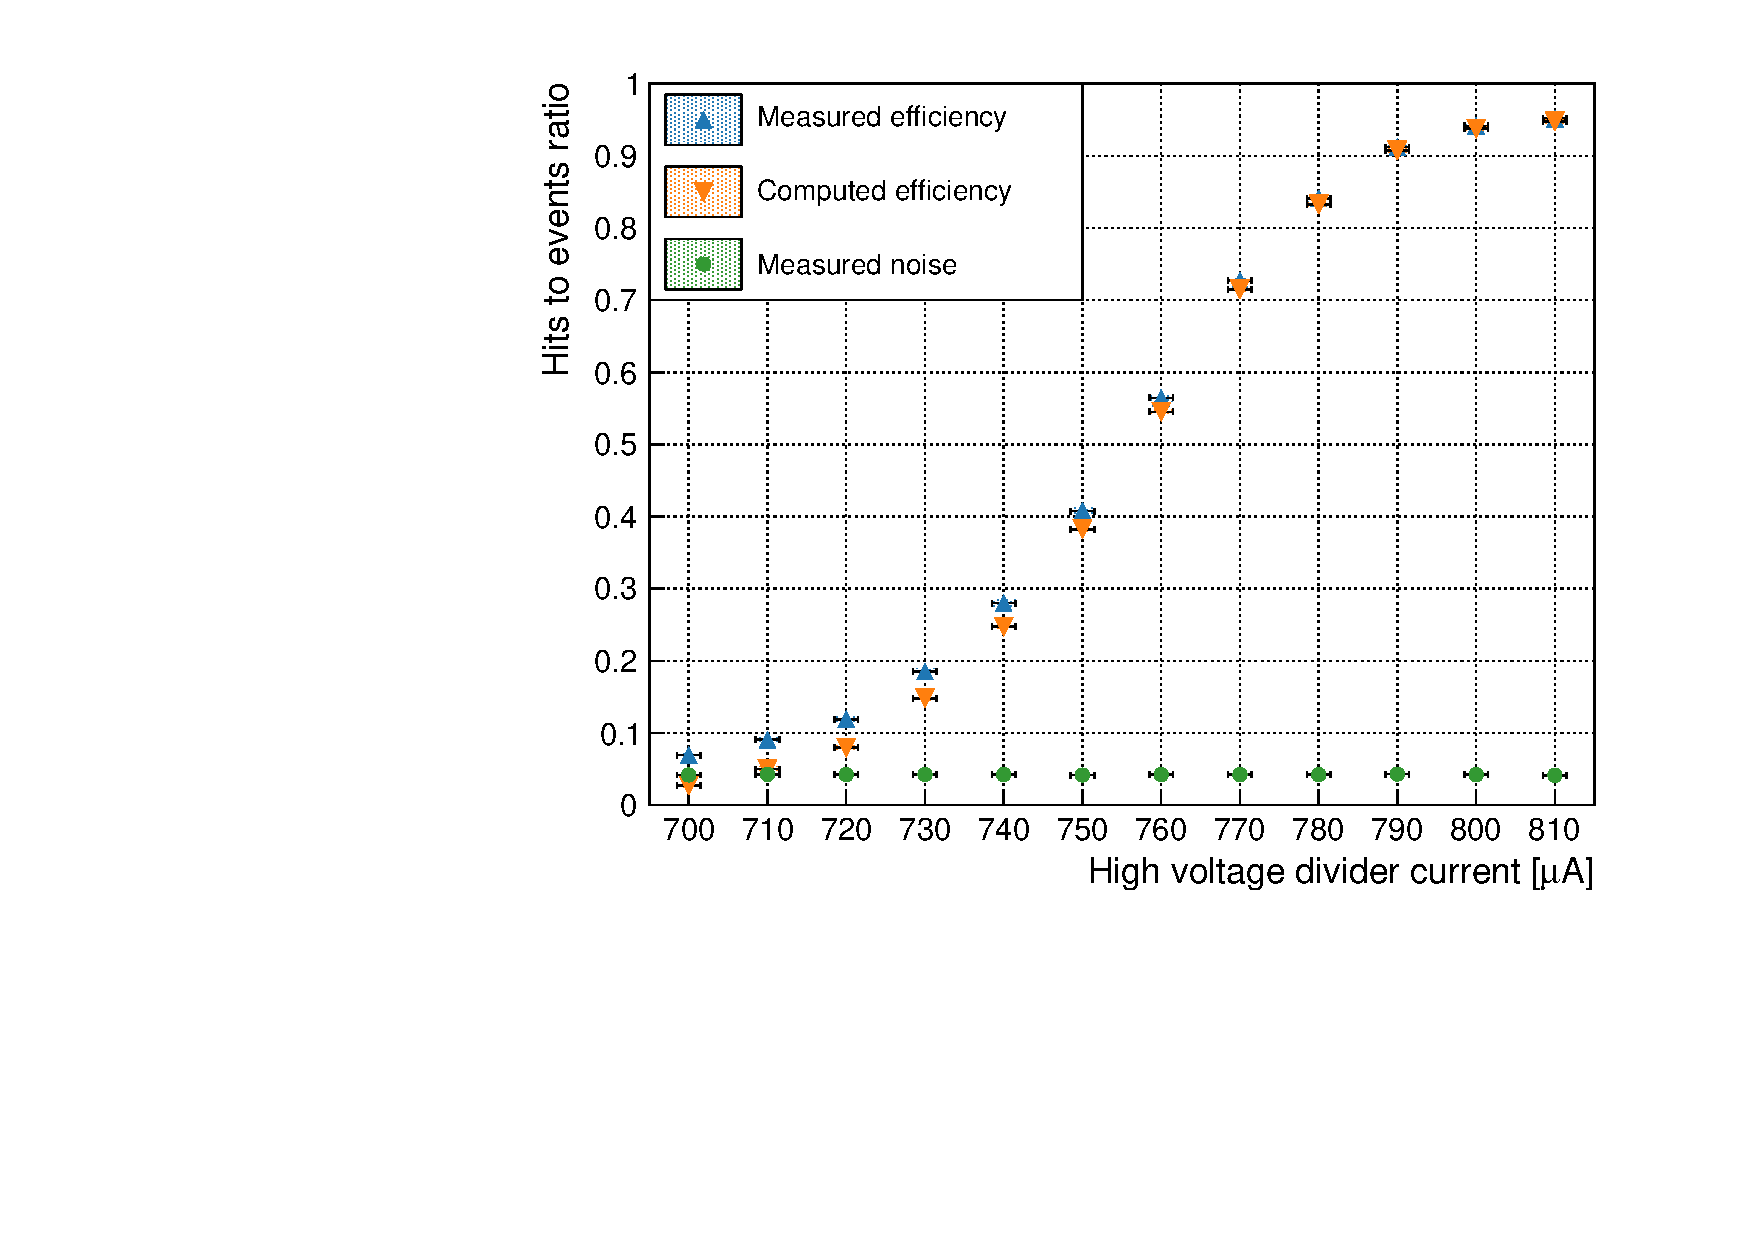
\includegraphics[width=0.49\textwidth]{img/plots/cEfficiency_HV_GEM1}
        \caption{Plots of the measured noise (green), measured efficiency (blue), and computed efficiency (orange) as a function of the high-voltage expressed in $\mu$A for GEM0 on the left and GEM1 on the right with muons.}
        \label{fig:II-3-data-eff-hv}
      \end{figure}

    \subsection{Efficiency against VFAT2 Threshold}

      Although it had been decided to run the system with a VFAT2 threshold of 25, a study of the evolution of the noise and efficiency according to the threshold was performed. It aimed at quantifiying the amount of noise and signal that was cut when increasing its value allowing to select the configuration yielding the best signal over noise ratio. Contrary to the previously operated scan which used trigger bits to measure the noise, this procedure uses tracking data and the full granularity information to analyze events. Figure \ref{fig:II-3-data-eff-threshold} plots the measured noise (green), measured efficiency (blue), and computed efficiency (orange) as a function of the VFAT2 threshold in terms of VFAT2 units for GEM0 on the left and GEM1 on the right with muons. Additionnal points in purple have been extracted from the tracking data. Using the two GEM detectors, it is possible to measure the efficiency of one using the other as reference. For each event, the following cuts were applied on the first GEM in order to reduce the dataset:
      \begin{itemize}
        \item only one cluster, group of adjacent strips that have been hit, is present in the event;
        \item the sole cluster must contain exactly two active strips;
        \item the center of the cluster must be at least ten strips away from the sides of the chip.
      \end{itemize}
      The first condition eliminates events where a hit is accompagnied by noise, creating an ambiguity on the cluster associated with the particles. The second condition helps to remove noise related events as they have a cluster size distribution peaked at one strip. Therefore, combining these two criteria creates a stringent condition for the selection of particle generated signals. The final condition ensures that the hit in the second GEM detector will be located inside the VFAT2 thus eliminate acceptance problems. Using the reduced dataset, the algorithm computed the efficiency by looking for hits in the second GEM detector in a window of five strips around the center of the cluster of the first GEM. \\

      \begin{figure}[h!]
        \centering
        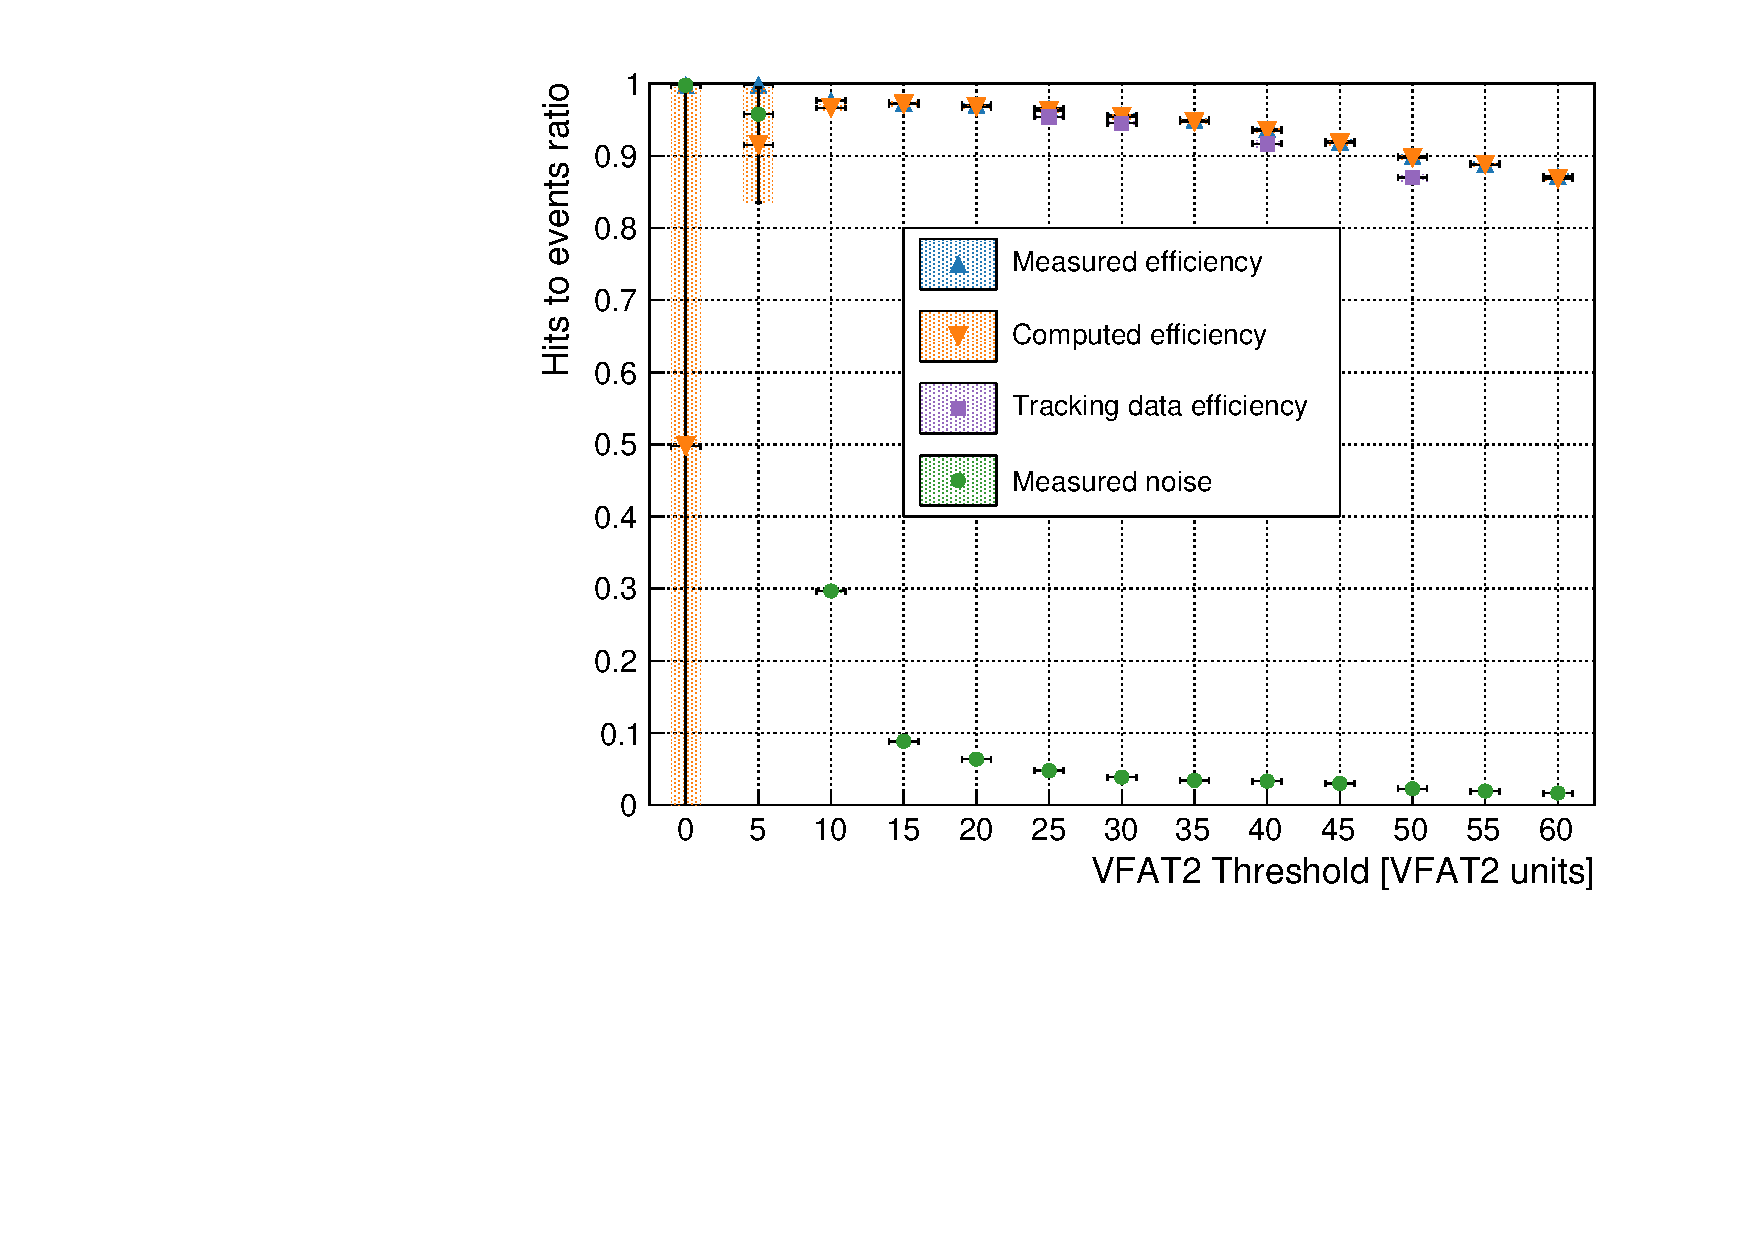
\includegraphics[width=0.49\textwidth]{img/plots/cEfficiency_Threshold_GEM0}
        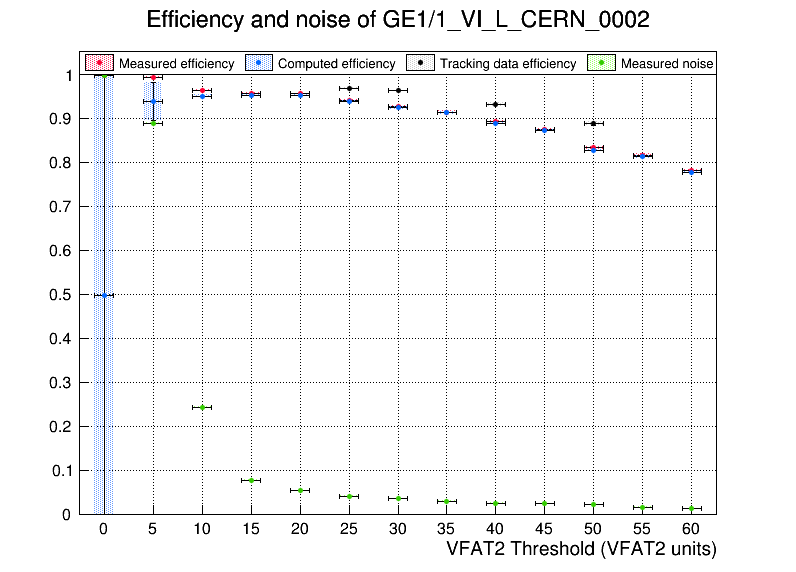
\includegraphics[width=0.49\textwidth]{img/plots/cEfficiency_Threshold_GEM1}
        \caption{Plots of the measured noise (green), measured efficiency (blue), computed efficiency (orange), and tracking data based efficiency (purple) as a function of the VFAT2 threshold in terms of VFAT2 units for GEM0 on the left and GEM1 on the right with muons.}
        \label{fig:II-3-data-eff-threshold}
      \end{figure}

      It can be seen that at very low thresholds the computed efficiency displays a large error due to the high noise. As the latter decreases with the increase in the threshold, the alogirthm computing the real efficiency is able to tighten its limits utlimatly providing a computed efficiency close to the measured value. From a threshold value of 15, efficiency starts to slowly drop reaching 90\% at 50. This shows how the threshold cuts the signal while only slightly affecting noise. From these results, the choice to operate the system at a threshold of 25 is validated. Although displaying a slightly lower efficiency, still around 97-98\%, than results at a threshold of 20, the lower noise is non-negligeable and reaches a local plateau.

      \todo{Deviation with tracking data}

    \subsection{Efficiency against Particle Rate}

      Similarly to the measurments and computations made for the previous study, the effect of particle rate on the efficiency was measured. Focus is given on the latter as it has been noted that noise levels are not influenced by the increase in rate. Figure \ref{fig:II-3-data-eff-rate} plots the measured efficiency (blue), computed efficiency (orange), and tracking data based efficiency (purple) as a function of the particle rates for GEM0 on the left and GEM1 on the right with pions. Control over the particle rates were done using collimaters in front of the beam setup. \\

      \begin{figure}[h!]
        \centering
        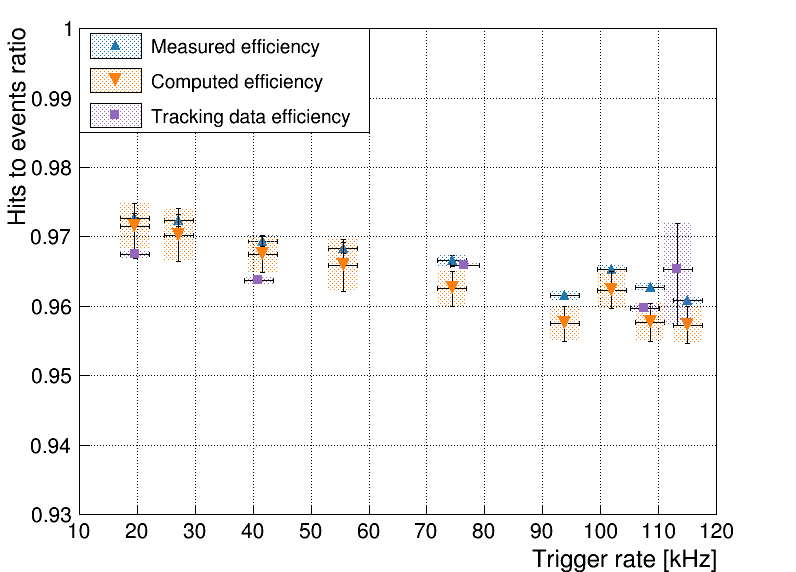
\includegraphics[width=0.49\textwidth]{img/plots/cEfficiency_Rate_GEM0}
        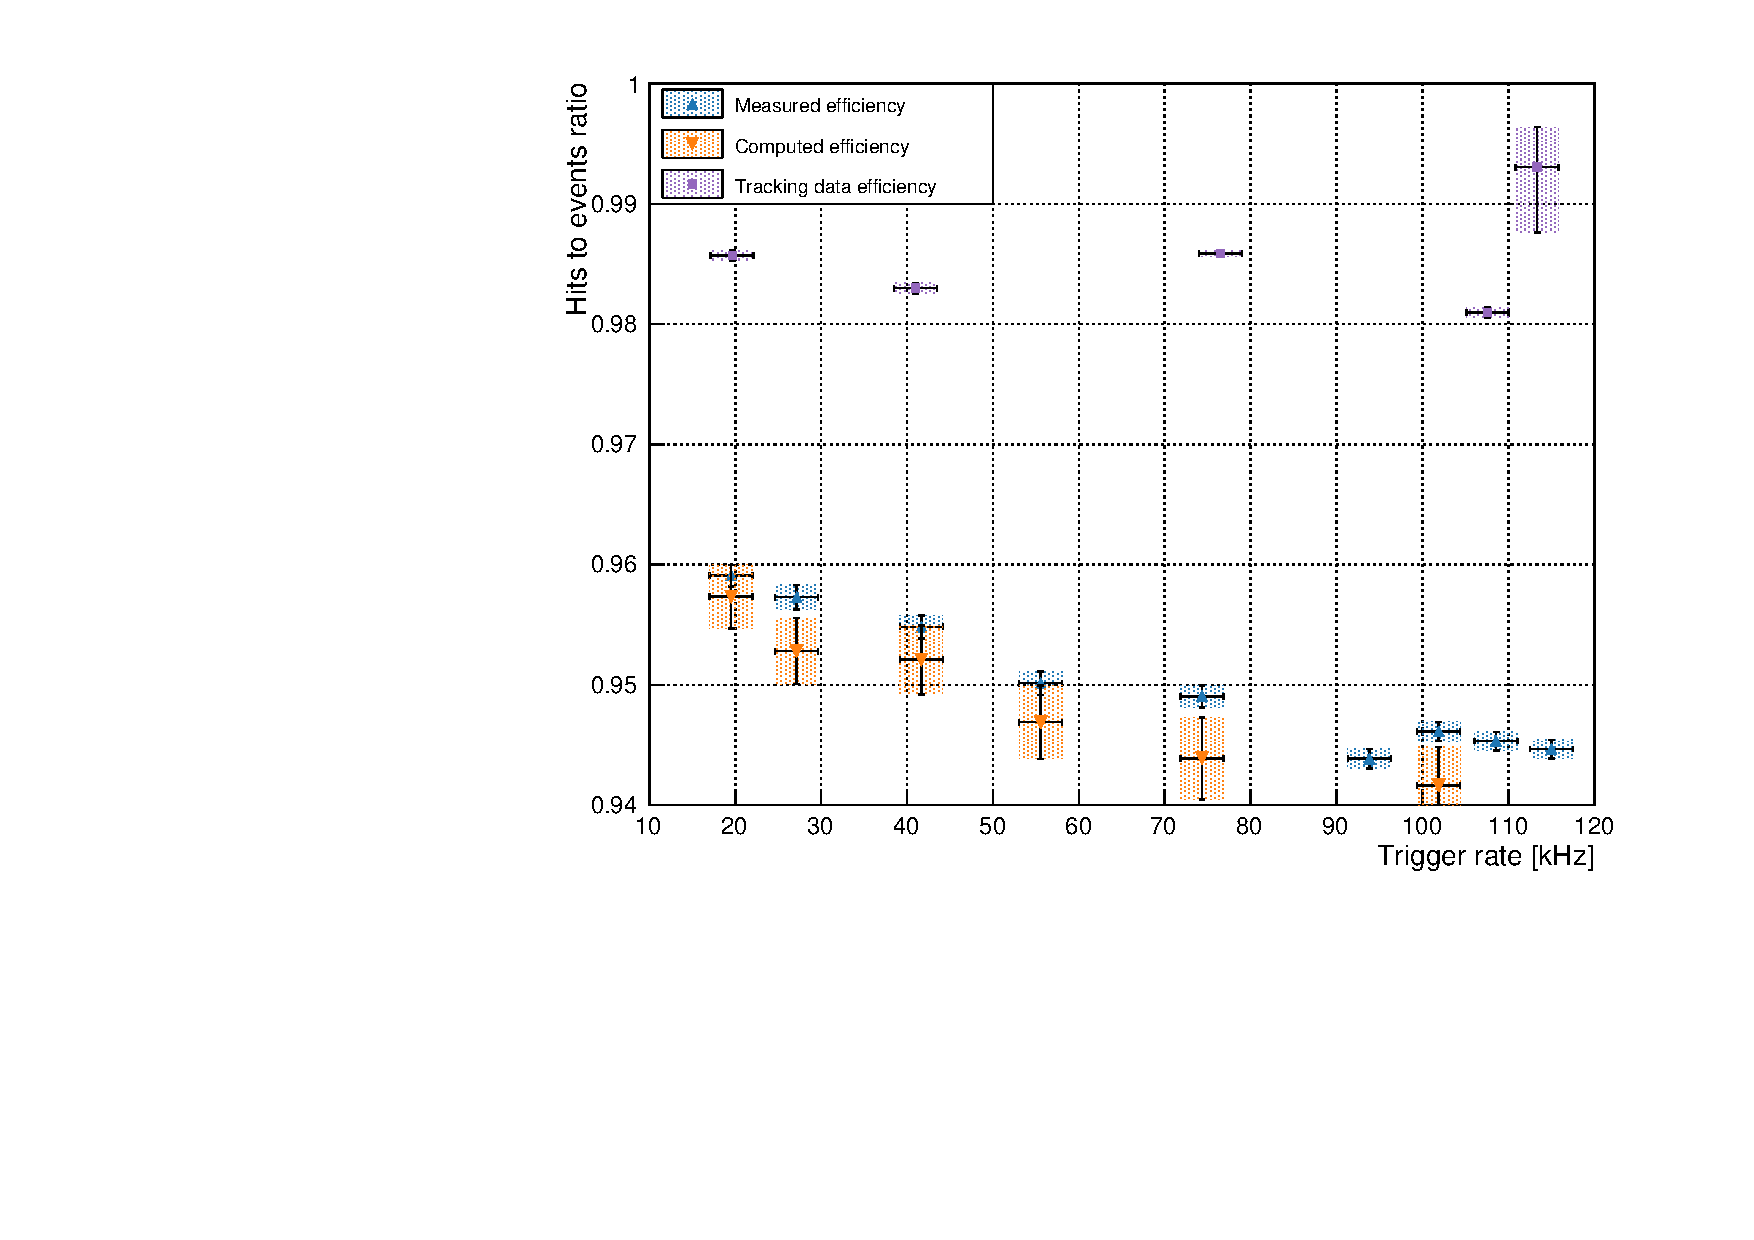
\includegraphics[width=0.49\textwidth]{img/plots/cEfficiency_Rate_GEM1}
        \caption{Plots of the measured efficiency (blue), computed efficiency (orange), and tracking data based efficiency (purple) as a function of the particle rates for GEM0 on the left and GEM1 on the right with pions}
        \label{fig:II-3-data-eff-rate}
      \end{figure}

      These results support the claim that GEM detectors can sustain rates up to several tens of kHz. When going from 20 kHz to 120 kHz, a drop in efficiency of 1\% is observed for GEM0 and of roughtly 2\% for GEM1.

      \todo{Deviation with tracking data}

    \subsection{Cluster Multiplicity and Size}

      Two studies that can be performed offline using the recorded data are the evolution of the cluster multiplicity, the number of clusters, and the cluster size, the number of strips per cluster, with the VFAT2 threshold. Figures \ref{fig:II-3-data-clu-mult} and \ref{fig:II-3-data-clu-size} respectivly plot the cluster multiplicity and cluster size for muons (green) and pions (blue) as a function of the VFAT2 threshold in terms of VFAT2 units for GEM0 on the left and GEM1 on the right.

      \begin{figure}[h!]
        \centering
        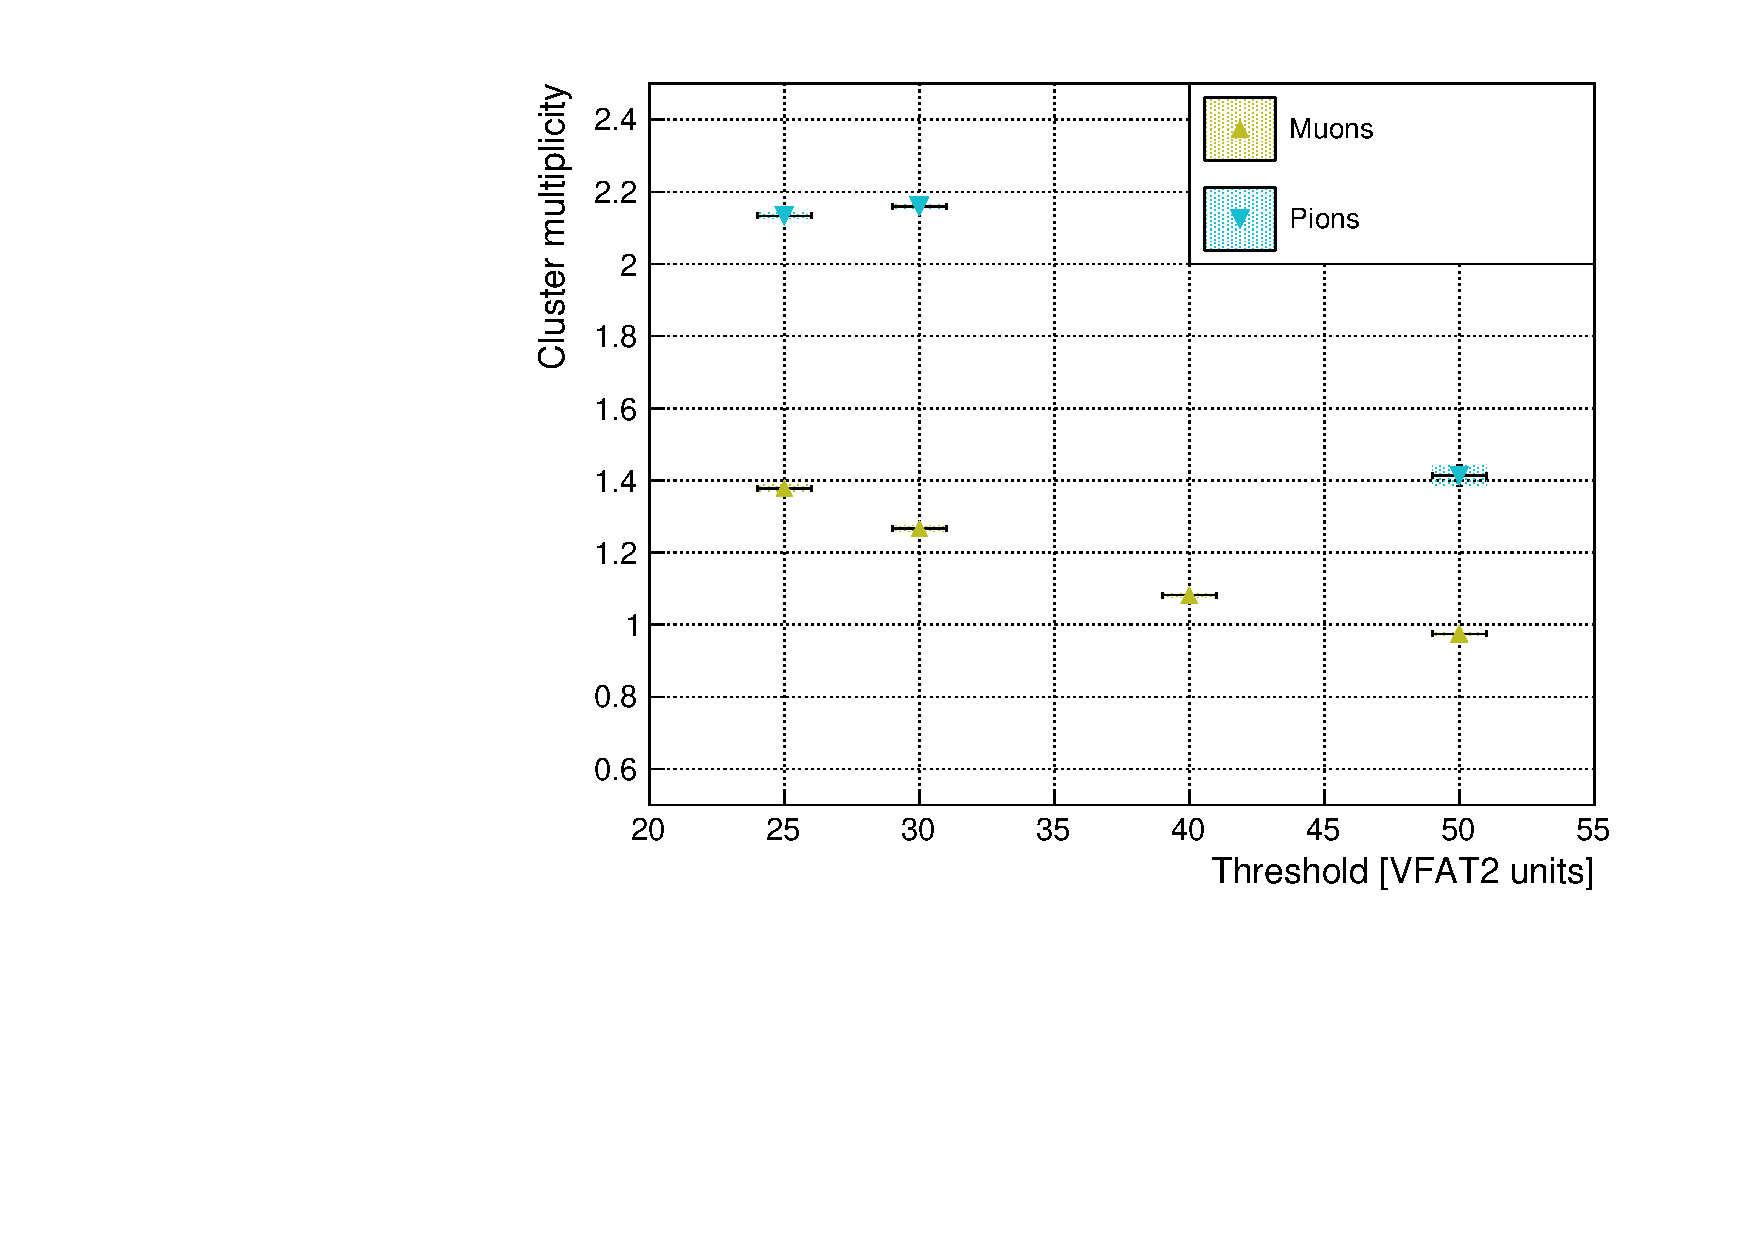
\includegraphics[width=0.49\textwidth]{img/plots/cClusterMultiplicity_Threshold_GEM0}
        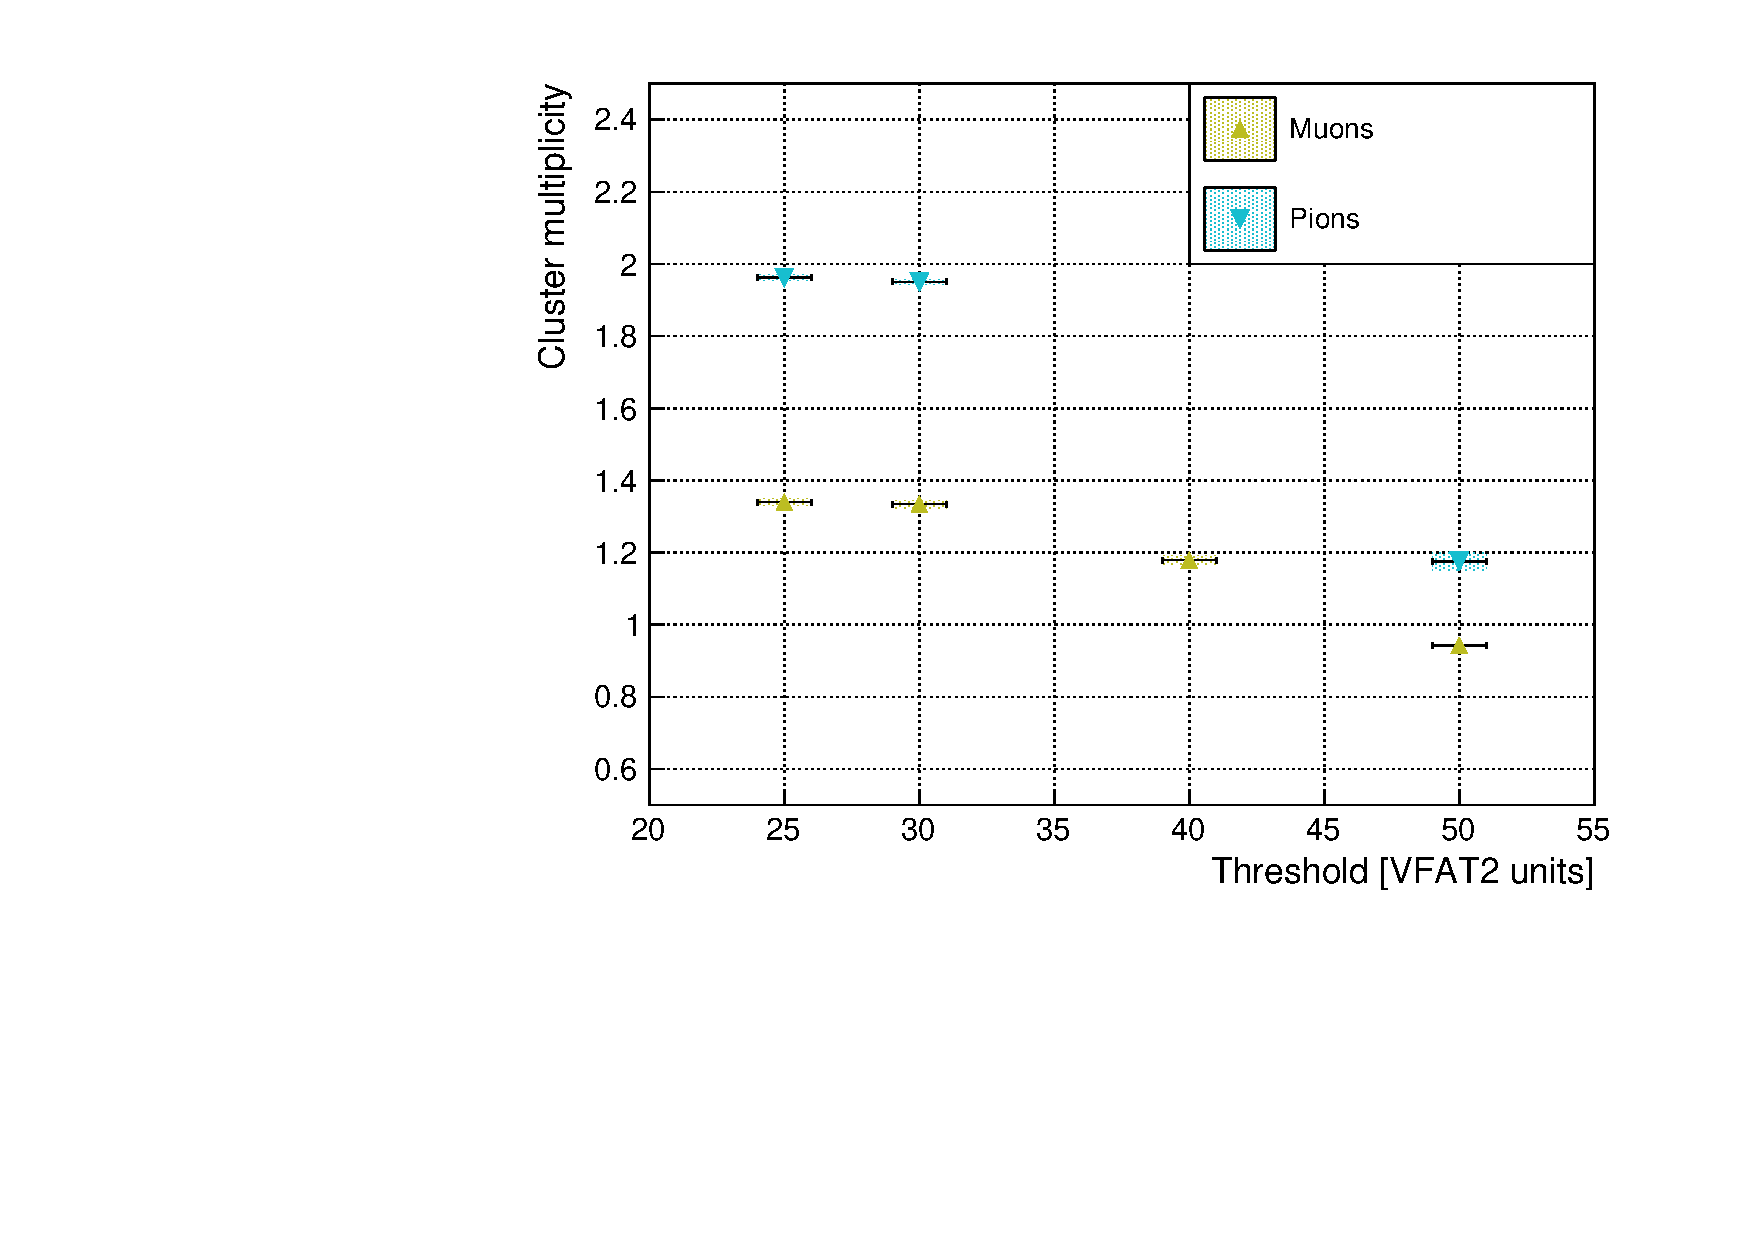
\includegraphics[width=0.49\textwidth]{img/plots/cClusterMultiplicity_Threshold_GEM1}
        \caption{???}
        \label{fig:II-3-data-clu-mult}
      \end{figure}

      \begin{figure}[h!]
        \centering
        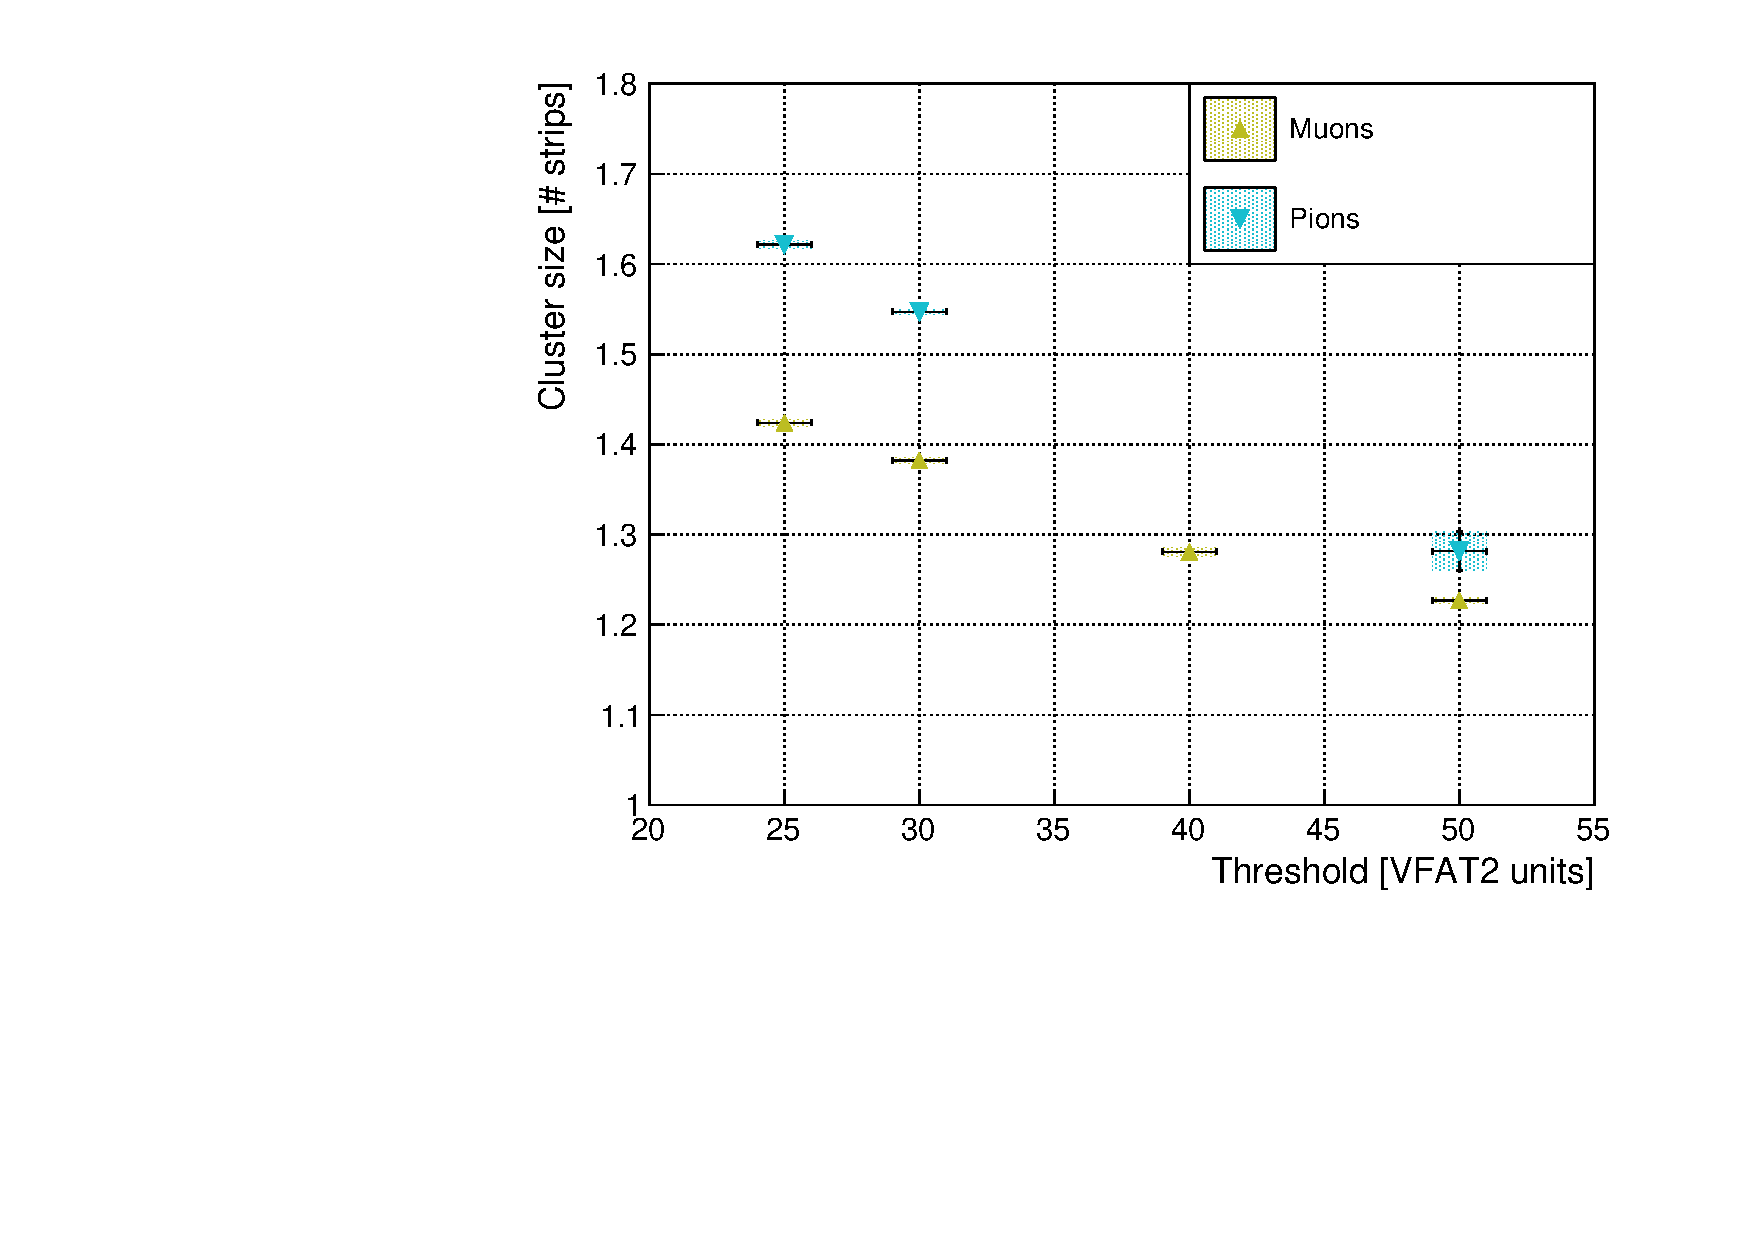
\includegraphics[width=0.49\textwidth]{img/plots/cClusterSize_Threshold_GEM0}
        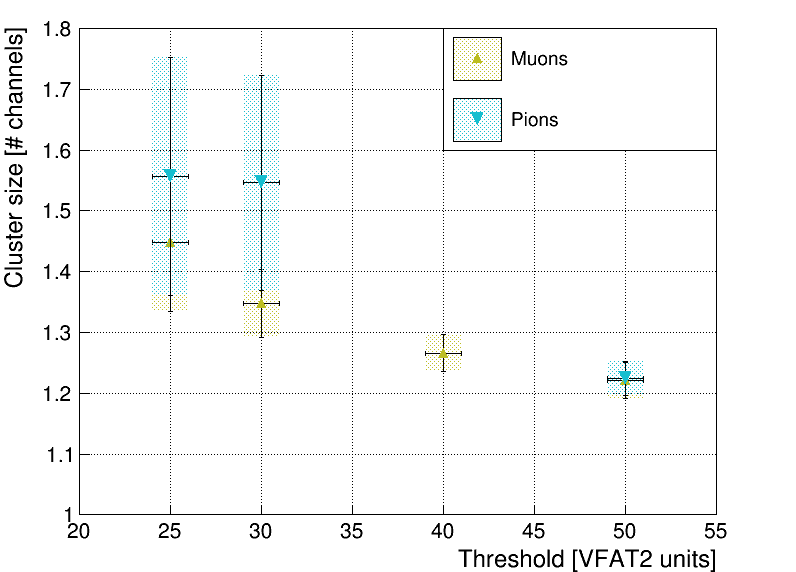
\includegraphics[width=0.49\textwidth]{img/plots/cClusterSize_Threshold_GEM1}
        \caption{???}
        \label{fig:II-3-data-clu-size}
      \end{figure}

    \subsection{Beam Profile}

      \begin{figure}[h!]
        \centering
        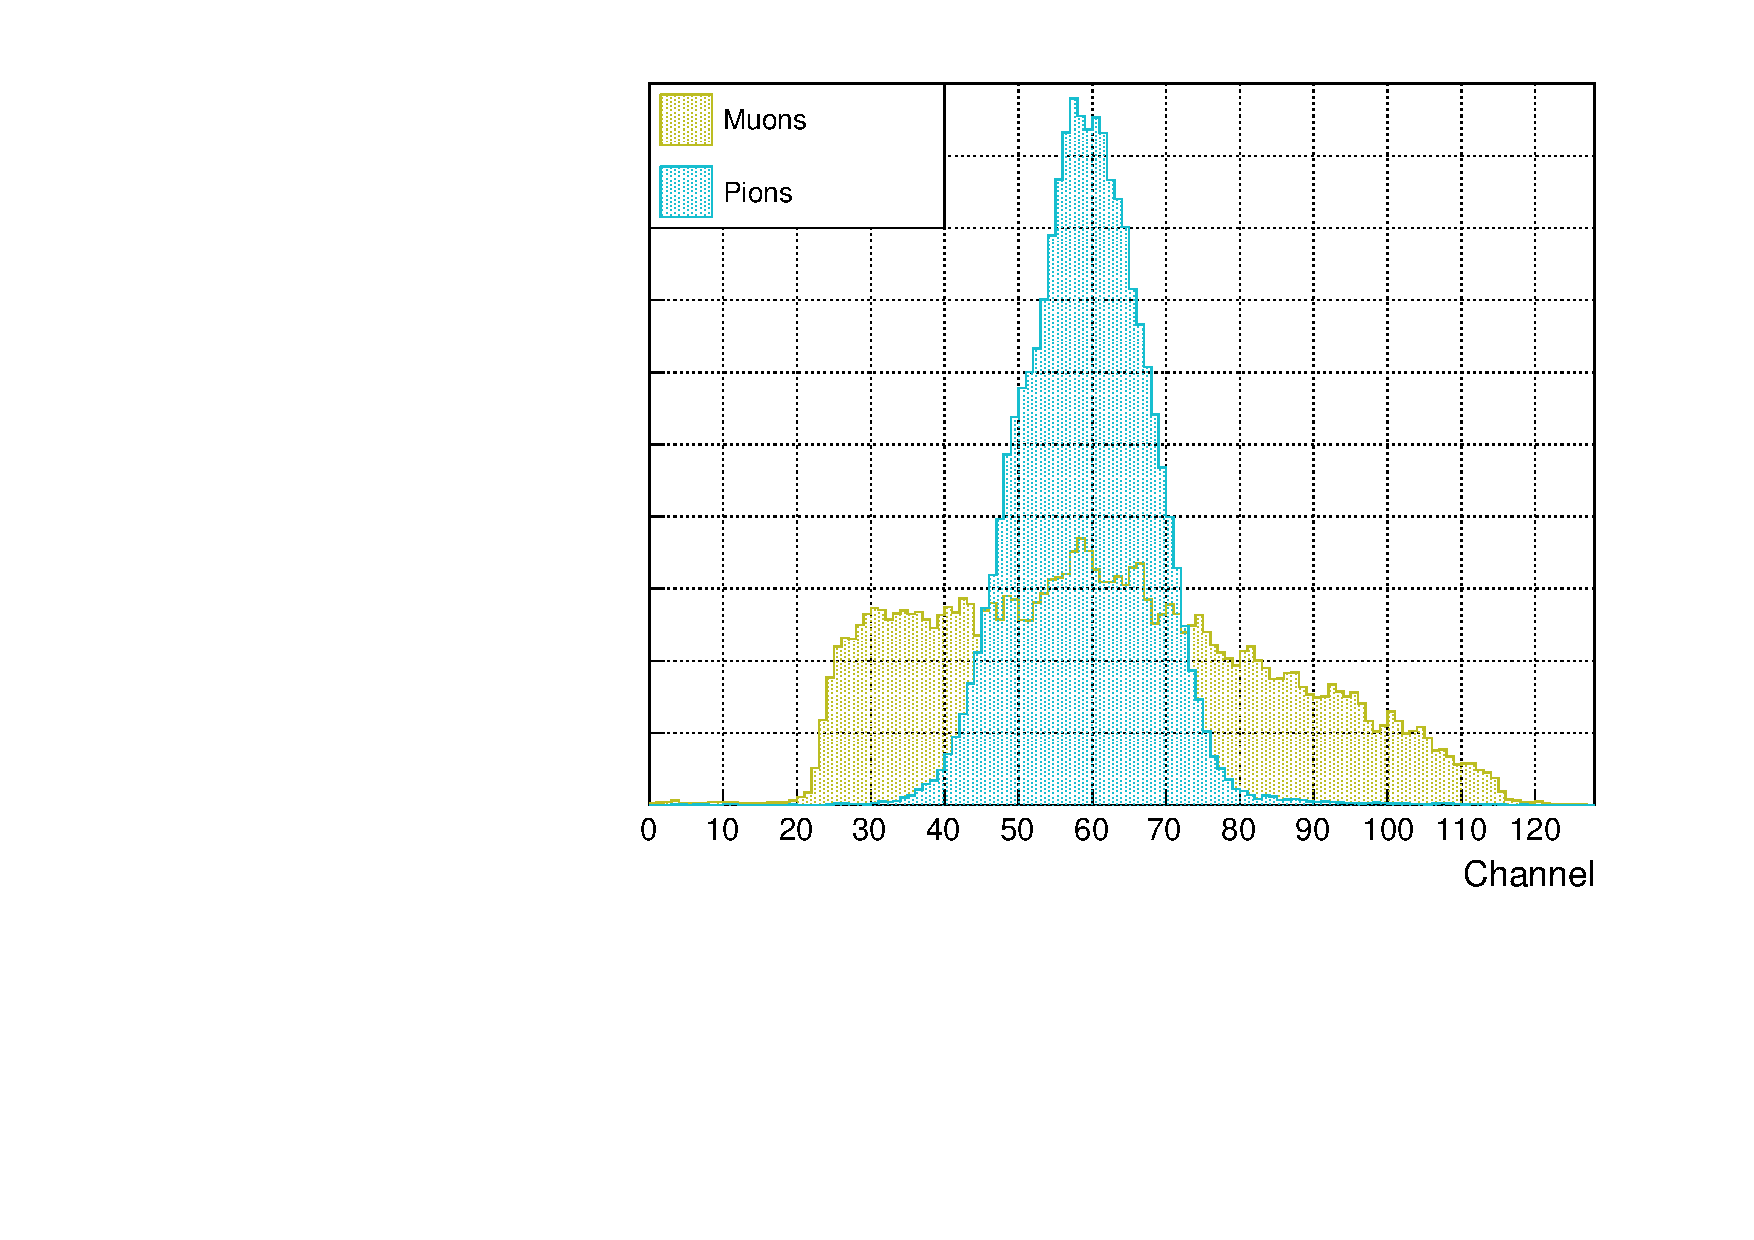
\includegraphics[width=0.49\textwidth]{img/plots/cBeamProfile_GEM0}
        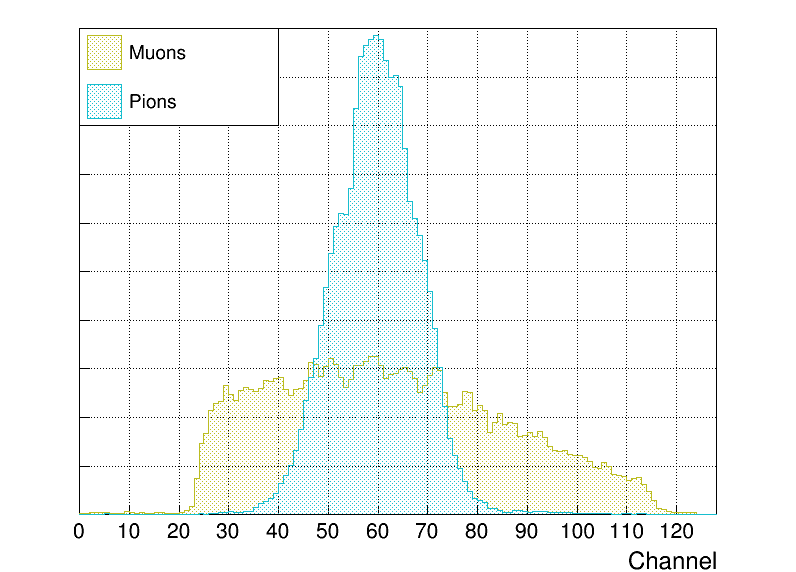
\includegraphics[width=0.49\textwidth]{img/plots/cBeamProfile_GEM1}
        \caption{???}
        \label{fig:II-3-data-beam-profile}
      \end{figure}

  \section{Conclusion}
